\documentclass[preprint,12pt]{elsarticle}
\usepackage{graphicx, xcolor, amsmath}
\usepackage{tabularx, booktabs, subcaption, longtable}
\usepackage{amssymb, url, newunicodechar, tikz}
\usepackage[utf8]{inputenc}
\graphicspath{{output/congested3/figures/}{output/congested3/}{output/paper-figures/}}
\newcolumntype{L}[1]{>{\raggedright\arraybackslash}p{#1}}
\newcolumntype{Y}{>{\raggedright\arraybackslash}X}
\usepackage[colorlinks=true,linkcolor=blue,citecolor=blue,urlcolor=blue]{hyperref}
\makeatletter
\g@addto@macro{\UrlBreaks}{\UrlOrds}
\makeatother
\Urlmuskip=0mu plus 2mu\relax
\emergencystretch=2em
\newunicodechar{−}{\ensuremath{-}}
\usetikzlibrary{
    positioning, % node distance, right=of, below=of
    shapes.misc, % rounded corners
    shapes.geometric, % ellipse nodes
    arrows.meta % arrow heads
}

\newunicodechar{₂}{$_2$}
\makeatletter
\def\ps@pprintTitle{%
 \let\@oddhead\@empty
 \let\@evenhead\@empty
 \def\@oddfoot{\centerline{\thepage}}%
 \let\@evenfoot\@oddfoot}
\newcommand{\stagecontent}[2]{%
  \parbox[c][2.35cm][c]{3.05cm}{%
    \centering
    \textbf{#1}\par
    \vspace{2mm}
    {\scriptsize #2\par}%
  }%
}
\makeatother

\begin{document}

\begin{frontmatter}

%% Title, authors and addresses

\title{Evaluating Data Centers as Assets in Local Energy Systems: A System-Integrated PUE Approach}

\author[usn]{Sambeet Mishra}
\author[usn]{Ankana Singha}
\author[usn]{Khaled Aleikish}
\author[usn]{Thomas {\O}yvang}
\author[bax]{Dominic Stephen}
\author[srnl]{Rob Hovsapian}

\address[usn]{University of South-Eastern Norway, Porsgrunn, Norway}
\address[bax]{Bax Innovation, Barcelona, Spain}
\address[srnl]{Savannah River National Laboratory, USA}


\begin{abstract}
Data centers can export waste heat, provide demand flexibility, and use storage to relieve local grid stress, yet Power Usage Effectiveness (PUE) treats the electricity consumed by these services as overhead. We introduce System-Integrated PUE (siPUE), which subtracts a single delay-adjusted, energy-equivalent credit from the PUE numerator. The credit reflects the monetized system value of heat recovery, flexibility, peak relief, and avoided carbon damage from a jointly optimized design. When no services are active, the credit is zero and siPUE reduces exactly to PUE. We evaluate the metric using a two-stage design-and-operation model for four data-center archetypes across ten shared uncertainty states, with explicit treatment of heat, flexibility, land, and construction delay. In all 40 canonical scenarios, service-active designs increase PUE. By contrast, siPUE is lower than the services-disabled comparator in 36 of 40 baseline scenarios and 23 of 40 scenarios for the shared min-max-regret design. Weighted by annual IT energy, the baseline design increases average PUE from 1.17 to 1.24 while reducing siPUE to 1.14; the robust design increases PUE to 1.34 while reducing siPUE to 1.15. The robust design delivers 10.56~EUR/MWh IT of delay-adjusted system benefit, equivalent to about 19\% of the reference electricity price. The reference price determines the magnitude of the credit, not its sign. Removing carbon damage from the ledger reverses the average improvement, indicating that both the magnitude and direction of the siPUE adjustment depend on the design objective and the assumed social cost of carbon. Internal property tests, held-out cases, and out-of-sample checks support the metric's internal consistency; external validation remains future work.
\end{abstract}

\begin{keyword}
Data centers \sep Power Usage Effectiveness \sep waste-heat reuse \sep optimization \sep local energy systems

\end{keyword}

\end{frontmatter}

\section*{Nomenclature}

\small
\setlength{\tabcolsep}{2pt}
\begin{longtable}{@{}L{0.13\linewidth} L{0.33\linewidth} L{0.12\linewidth} L{0.32\linewidth}@{}}
\toprule
\multicolumn{4}{@{}l}{\emph{Metric terms}} \\
\midrule
$\text{PUE}$ & Power Usage Effectiveness, $E_{\text{FAC}}/E_{\text{IT}}$ & $B_{\text{sys}}$ & Credited system benefit (EUR/yr) \\
$\text{siPUE}$ & System-Integrated PUE & $C_{\text{ind}}$ & Independent system-cost ledger (EUR/yr) \\
$E_{\text{FAC}}$ & Facility electricity (MWh/yr) & $E_{\text{credit}}$ & Delay-adjusted energy credit (MWh/yr) \\
$E_{\text{IT}}$ & Delivered IT electricity (MWh/yr) & $p_{\text{ref}}$ & Frozen reference price (EUR/MWh) \\
$C_{\text{el}}, C_{\text{trans}}$ & Electricity-resource, network cost (EUR/yr) & $a_s$ & Lifecycle availability factor, $a_s\in[0,1]$ \\
$C_{\text{peak}}$ & Peak-capacity cost (EUR/yr) & $[z]^+$ & Positive part, $\max(0,z)$ \\
$C_{\text{CO2,dam}}$ & Carbon-damage cost (EUR/yr) & $0, d$ & Superscripts: comparator, design \\
$V_{\text{heat}}, V_{\text{flex}}$ & Avoided heat, flexibility cost (EUR/yr) & & \\
\midrule
\multicolumn{4}{@{}l}{\emph{Design and optimization}} \\
\midrule
$x, \hat{x}$ & Design variables, shared robust design & $C_s, C_s^{\star}$ & Lifecycle market cost, scenario optimum \\
$y_s$ & Hourly operational variables in state $s$ & $R_s$ & Normalized regret \\
$s\in\mathcal{S}$ & Shared uncertainty state & $Z$ & Worst-case regret \\
$K_{\text{HX}}, K_{\text{HP}}$ & Heat-exchanger, heat-pump capacity & & \\
\midrule
\multicolumn{4}{@{}l}{\emph{Carbon accounting and regret normalization}} \\
\midrule
$\text{Cap}^{\text{applied}}_s$ & Applied carbon cap (tCO2) & $\text{Cap}^{\text{policy}}_s$ & Policy-target carbon cap (tCO2) \\
\multicolumn{2}{@{}L{0.46\linewidth}}{$E^{\text{services-disabled}}_{s,\min}$: comparator's minimum achievable emissions (tCO2)} & $\epsilon$ & Regret-normalization floor \\
$E_{\text{IT},s}^{\text{PV}}$ & PV-discounted lifetime IT energy (MWh) & $k$ & Reference-price multiplier, $\text{siPUE}(k)$ \\
$\phi$ & Flexible-load fraction & $\alpha^{\text{base}}$ & Base cooling-overhead ratio (pre-retrofit) \\
\midrule
\multicolumn{4}{@{}l}{\emph{Appendix: network, heat, and storage parameters}} \\
\midrule
$F_{12}, F_{23}$ & DC power flow, node pairs 1--2, 2--3 (MW) & $F_{13}$ & DC power flow, node pair 1--3 (MW) \\
$E^{\text{co2}}$ & Physical emissions (tCO2) & $n$ & Network node index \\
$t, T$ & Hour index; total representative hours & $\Delta t, w_t$ & Timestep (h); cluster weight \\
$\varepsilon^{\text{th}}_n$ & Node thermal emission factor & $G^{\text{th}}_{n,t}$ & Thermal generation, node $n$, hour $t$ (MW) \\
$\varepsilon^{\text{boil}}$ & Boiler emission factor (tCO2/MWh$_{\text{th}}$) & $D^{\text{dh}}_t$ & District-heating demand, hour $t$ (MWh$_{\text{th}}$) \\
$H^{\text{sold}}$ & Delivered (sold) heat (MWh$_{\text{th}}$) & $K$ & District-heating price segments (count) \\
$\lambda^{\text{th}},\eta^{\text{th}}$ & Thermal-store self-discharge, round-trip efficiency & $\eta^{\text{ch}},\eta^{\text{dis}}$ & Battery charge, discharge efficiency \\
$\gamma^{\text{ups}}$ & UPS reserve-floor fraction & & \\
\bottomrule
\end{longtable}

\begin{sloppypar}
\noindent\emph{Abbreviations.} CUE, Carbon Usage Effectiveness; DC-OPF, direct-current optimal power flow; DCRE, Data Centre Resource Effectiveness; DESS, Data centre Environmental Sustainability Score; DH, district heating; ERF/ERE, Energy Reuse Factor/Effectiveness; ETS, Emissions Trading System; HX, heat exchanger; HP, heat pump; REF, Renewable Energy Factor; WUE, Water Usage Effectiveness.
\end{sloppypar}
\normalsize

\section{Introduction}
\label{sec:introduction}

Electricity demand from European data centers has become a material consideration in transmission and distribution planning. Commission estimates put EU consumption at 76.8~TWh in 2018, with projections of 98.5~TWh by 2030 under a trend case and up to 160~TWh under a high-growth case \cite{1}; more recent assessments suggest roughly 96~TWh in 2024 and nearly 168~TWh by 2030 \cite{2}. Traffic growth and compute-intensive AI workloads reshape annual demand, ramping behavior, peak demand, heat rejection, cooling requirements, and flexibility headroom \cite{14,19}.

At this scale, data-center expansion becomes a local infrastructure and investment challenge. Connection rights, congestion, heat offtake, flexibility-market eligibility, land-use approvals, permitting timelines, and community acceptance increasingly determine which projects proceed \cite{6,21}. The EU energy transition creates an additional set of pressures. Electricity and heat systems need flexibility, digital coordination, and sector coupling \cite{7,8}, while sustainability reporting for large data centers is being formalized through Directive (EU) 2023/1791 and sector initiatives \cite{15,16}. Data centers can therefore act either as inflexible loads or as service-active assets that export waste heat, provide grid support, and manage dynamic AI-driven loads \cite{11,13}.

A key reporting limitation is that PUE evaluates only internal electricity overhead. Heat pumps, heat exchangers, controllability, storage, and telemetry can increase facility electricity consumption even when they reduce local system cost. This creates the KPI gap studied here. PUE captures the facility-energy burden, whereas the independent system-cost benefit lies outside the metric boundary. siPUE is introduced as an indicator, expressed in PUE's own energy units, that translates that benefit into an adjustment to the PUE numerator while preserving PUE's internal-efficiency role.

\subsection{Related Work}
\label{sec:related}

The relevant literature spans data-center metrics, heat recovery, flexibility, integrated energy systems, and robust decision-making. PUE remains the dominant facility-efficiency ratio \cite{Belady2008PUE,greengrid2014}, but critiques show that it omits flexibility, source effects, climate dependence, and wider sustainability dimensions \cite{Reddy2017,VandeVoort2017}. Parallel indicators such as CUE (Carbon Usage Effectiveness), WUE (Water Usage Effectiveness), ERF/ERE (Energy Reuse Factor/Effectiveness), and REF (Renewable Energy Factor) capture additional dimensions under the ISO 30134 family and EU reporting practice \cite{ISO30134,EUDataCenterDirective2023}, but they do not provide a market-valued PUE numerator credit.

Waste-heat and district-heating studies establish data-center heat as a measurable system service \cite{11,10}, while demand-response and flexibility studies show that IT load, cooling, and batteries can provide grid services under suitable market rules \cite{Takci2025,Crozier2025}. Integrated energy-system papers quantify these services within optimization models and show potential cost or emissions reductions \cite{JerezMonsalves2023,Wang2024}. These studies motivate system valuation but leave a standalone reporting question: how should an operator report a service-active design when PUE rises because the service itself consumes electricity?

Broader scoring approaches, including DESS and DCRE, broaden the resource and contextual boundaries \cite{Terenius2023,GreenGrid2025DCRE}, and recent heat and flexibility reviews reinforce the need for quantifiable energy-system indicators \cite{Yuan2025,Takci2025}. The combined, delay-adjusted heat, flexibility, peak, and carbon-damage value of a jointly optimized design is not captured by a PUE-normalized reporting metric.

An established robust-optimization framework serves as the uncertainty test bed. Minimizing worst-case regret follows the min-max-regret tradition \cite{savage1951theory,MR-1626-RPC}. Accordingly, the methodological claim is limited to comparing the PUE and siPUE responses of the same normalized min-max-regret design.

\subsection{Synthesis and Gap Identification}

Table~\ref{tab:metric-novelty-comparison} positions the proposed metric against the most closely related reporting metrics and integrated-energy-system modeling literature. The contribution is an accounting translation of local-system value into a PUE numerator credit.

\begin{table}[tbp]
\centering
\scriptsize
\setlength{\tabcolsep}{3pt}
\renewcommand{\arraystretch}{1.12}
\caption{Comparison of siPUE with adjacent data-center metrics and modeling approaches. WUE (Water Usage Effectiveness) and REF (Renewable Energy Factor) are omitted from the table: neither assigns monetary value to energy-system services, so both differ from siPUE in the same way that CUE does.}
\label{tab:metric-novelty-comparison}
\begin{tabularx}{\linewidth}{L{2.05cm} L{2.25cm} L{1.65cm} L{1.85cm} Y}
\toprule
Approach & Primary function & Values local-system services? & PUE numerator credit? & Gap relative to siPUE \\
\midrule
PUE \cite{Belady2008PUE,EUDataCenterDirective2023} & Facility electricity divided by IT electricity & No & Baseline ratio & Treats heat-pump, storage, and control electricity as overhead even when they create external value. \\
ERF/ERE \cite{EUDataCenterDirective2023} & Reused-energy reporting and energy-reuse effectiveness & Heat only, in energy terms & Partial reuse adjustment & Omits flexibility, peak, network, carbon-damage, and delay effects. \\
CUE \cite{Reddy2017} & Carbon emissions per IT energy & Carbon footprint only & No & Parallel intensity indicator; no numerator credit. \\
DESS \cite{Terenius2023} & Broader sustainability score & Partial, contextual & No & Qualitative and contextual; no numerator credit. \\
DCRE \cite{GreenGrid2025DCRE} & Resource-effectiveness view of energy, water, water stress, and climate context & Indirect & No & Broader resource boundary; no numerator credit. \\
Integrated energy-system optimization papers \cite{JerezMonsalves2023,Wang2024} & System-cost or emissions optimization & Yes, inside the model & No & Quantifies system impacts while leaving standalone reporting-compatible numerator credits undefined. \\
siPUE (this study) & Numerator credit for service-active data centers & Yes: heat, flexibility, peak, and carbon damage, adjusted for construction delay & Yes & Converts the independent system-cost benefit into an energy-equivalent numerator credit and reduces to PUE when no services are active. \\
\bottomrule
\end{tabularx}
\end{table}

Across this literature, the remaining gap is an accounting one. Current reporting metrics either measure one dimension or widen the resource boundary without translating local-system services into PUE's own energy units. Heat reuse, flexibility, and carbon impacts are also seldom valued with empirical electricity, heat, reserve, or ETS prices. None of the reviewed approaches translates the combined, delay-adjusted value of a jointly optimized design's heat, flexibility, peak, and carbon-damage effects into the PUE numerator.

\subsection{Conceptual Framework and Research Questions}
Energy-system context, data-center design decisions, and local energy-system outcomes are linked in the analysis. Policy documents, market data, and industry practice supply the institutional context summarized in Section~\ref{sec:policy-context}; the model in Section~\ref{sec:methodology} provides the basis for the structured, testable claims. The resulting model-based research questions are:
\begin{enumerate}
\item RQ1: Can an indicator, expressed in PUE's own energy units, reveal the combined local-system value that a jointly optimized design creates through heat, flexibility, peak, and carbon damage, adjusted for construction delay, while reducing exactly to PUE when no services are active?
\item RQ2: How do shared min-max-regret design decisions affect traditional efficiency metrics and system-integrated indicators?
\end{enumerate}

The min-max-regret design is treated as an uncertainty test bed, with validation of the investment rule left outside the scope of this study.


\subsection{Contributions}
siPUE is introduced as an indicator that converts local-system benefit into a PUE numerator credit. Its boundary, normalization, and reference-price rules define the conversion from monetized system value to energy-equivalent credit. The metric is tested in a two-stage model that combines scenario-perfect benchmarks with a shared normalized min-max-regret design and explicit treatment of lifecycle delay, carbon, land, heat recovery, flexibility, storage, and DC-OPF network constraints. The evaluation spans four archetypes and ten shared uncertainty states, decomposes the credit by ledger component, and reports sensitivity to price, technology, land, and delay assumptions.

\section{Data Centers in Local Energy Systems --- Policy and Market Context}
\label{sec:policy-context}

Data-center integration depends on macro-level policy, meso-level infrastructure, and micro-level project finance. A service-active project is most viable when these levels align, as summarized in Figure~\ref{fig:macro-meso-micro}.

\begin{figure}[tbp]
\centering
\footnotesize
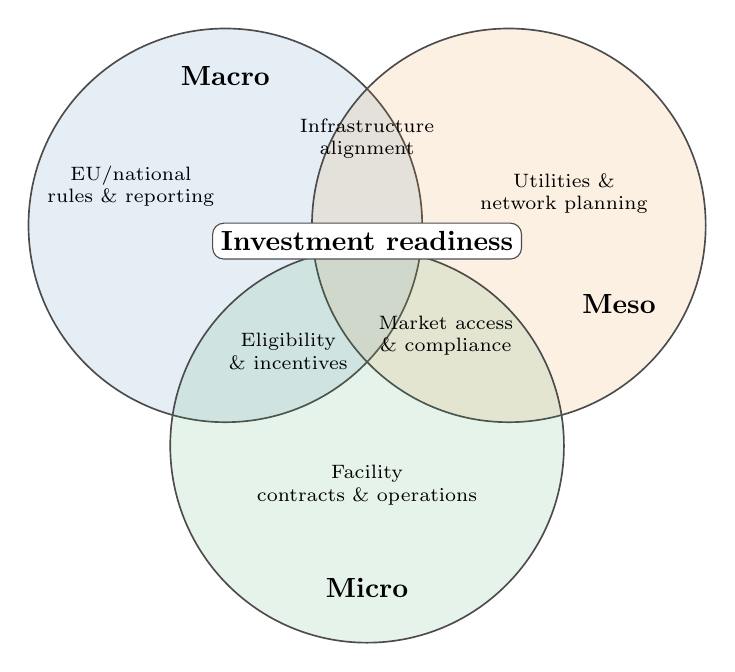
\begin{tikzpicture}

\def\r{2.5}

\definecolor{macrocol}{RGB}{52,120,180}
\definecolor{mesocol}{RGB}{230,140,40}
\definecolor{microcol}{RGB}{60,160,90}

\coordinate (A) at (0,0);
\coordinate (B) at (3.6,0);
\coordinate (C) at (1.8,-2.8);


\draw[line width=0.6pt, draw=black!70, fill=macrocol, fill opacity=0.13] (A) circle (\r);
\draw[line width=0.6pt, draw=black!70, fill=mesocol,  fill opacity=0.13] (B) circle (\r);
\draw[line width=0.6pt, draw=black!70, fill=microcol, fill opacity=0.13] (C) circle (\r);


\node at (0,1.9) {\textbf{Macro}};
\node at (5.0,-1) {\textbf{Meso}};
\node at (1.8,-4.6) {\textbf{Micro}};


\node[align=center, font=\scriptsize] at (-1.2,0.5)
{EU/national\\rules \& reporting};

\node[align=center, font=\scriptsize] at (4.3,0.4)
{Utilities \&\\network planning};

\node[align=center, font=\scriptsize] at (1.8,-3.3)
{Facility\\contracts \& operations};

\node[align=center, font=\scriptsize] at (1.8,1.1)
{Infrastructure\\alignment};

\node[align=center, font=\scriptsize] at (0.8,-1.6)
{Eligibility\\\& incentives};

\node[align=center, font=\scriptsize] at (2.8,-1.4)
{Market access\\\& compliance};


\node[draw=black!70, rounded corners, fill=white, inner sep=3pt]
at (1.8,-0.2)
{\textbf{Investment readiness}};

\end{tikzpicture}
\caption{Conceptual macro--meso--micro governance structure. Investment readiness emerges when regulatory signals, infrastructure feasibility, and project-level execution align. This structure is adapted from the multi-level perspective in socio-technical transitions literature \cite{GEELS2020119894} to fit the data-center energy-integration context.}
\label{fig:macro-meso-micro}
\end{figure}

At the macro level, the recast Energy Efficiency Directive imposes reporting obligations on large data centers and codifies PUE, Renewable Energy Factor, and Energy Reuse Factor \cite{15}. The accompanying delegated regulation sets the reporting template \cite{EUDataCenterDirective2023}, and the Climate Neutral Data Centre Pact adds voluntary renewable-supply and heat-reuse targets \cite{16}. The Green Deal and the ``Fit for 55'' package increase the economic value of efficiency, waste-heat reuse, and flexibility \cite{17,7}. The action plan on digitalizing the energy system treats flexibility, interoperability, and data availability as prerequisites for renewable integration \cite{8}. Carbon pricing reinforces these incentives. By raising the marginal cost of fossil generation, EU ETS prices increase the relative value of demand reduction, heat reuse, and electrified heat \cite{7}. Because these KPIs now feature in due diligence, ESG scoring, and financing conditions \cite{EUDataCenterDirective2023}, a metric boundary that omits system services can distort investment signals.

At the meso level, grid capacity is usually the binding constraint. Large steady loads can trigger reinforcement, congestion charges, import caps, or paused connection queues \cite{6,21}. Projects that credibly reduce peak stress may therefore be better positioned in permitting and connection negotiations. Land and heat-network access constrain projects in parallel, since integration equipment expands the footprint and heat value depends on network proximity, temperature requirements, pipe capacity, and tariff treatment \cite{11,23}. Timing is a major meso-level risk. Data centers can be built faster than grid reinforcements or district-heating extensions, so service revenue may arrive after capital is committed. The geography of renewable resources further shapes this pattern. Nordic and energy-hub settings can improve cooling-overhead and heat-cascading economics, while dense urban clusters offer heat demand but tighter grid and land constraints \cite{24,25}.

At the micro level, heat exchangers, heat pumps, storage, controllability, and telemetry raise capital costs but can diversify revenue streams. Contracted heat or flexibility revenue can support lower-cost debt financing, whereas uncertain service revenue may shift financing toward equity, which can encourage staged integration: connection rights or heat offtake are secured first, while additional storage or controllability is deferred \cite{23,12}. Because PUE and related KPIs enter the same due-diligence process, projects that add integration electricity can look weaker precisely when they create system value \cite{Belady2008PUE,VandeVoort2017}.

Local-system value can be monetized only where a service can be contracted and measured. Heat recovery uses 25--40$^\circ$C cooling streams and heat exchangers or heat pumps to reach district-heating or process-heat temperatures; commercial value depends on offtake contracts, tariffs, and responsibility for temperature lift \cite{11,22,23}. Electrical flexibility comes from controllable IT and cooling load and from batteries installed for reliability, whose value depends on product definitions, telemetry, settlement rules, grid-access conditions, and congestion risk \cite{13,Takci2025,Crozier2025}. Renewable procurement and energy-hub co-location can anchor siting decisions, but their value remains place-specific because land, grid access, and heat-network proximity determine where integration can be realized \cite{24,25,9}.

Integration can stall when reporting, infrastructure planning, and financing signals diverge. A project can satisfy decarbonization policy while still facing grid-connection limits, spatial constraints, or uncertain service cash flow. PUE remains the dominant reporting metric \cite{ISO30134,Belady2008PUE}, but it classifies all non-IT electricity as overhead. Heat pumps, storage, and controllable cooling therefore worsen PUE even when they create external value \cite{VandeVoort2017,Reddy2017}. The siPUE metric preserves the PUE numerator and denominator logic and adds a separate credit for monetized local-system benefits, leaving private revenues and costs outside the credit. The model adopts the same accounting boundary. IT demand follows the workload profiles, and delay enters through lifecycle availability. Electricity-side constraints use hourly balance and a three-node DC-OPF. Heat, flexibility, storage, carbon, land, and lease costs are represented through explicit physical and accounting terms.


\section{Method: siPUE definition and two-stage model}
\label{sec:methodology}

siPUE and the optimization framework used to test it are defined in this section. The PUE structure is retained, while the independent system-cost benefit is translated into an energy-equivalent numerator credit. The benefit includes avoided resource, transmission, peak, and carbon-damage cost; private heat and flexibility revenue remain in the market-cost objective.

The model evaluates capital decisions for heat exchangers, heat pumps, flexibility capacity, batteries, and land together with hourly operation. It also includes a locked 15\% efficiency retrofit, defined in Appendix A.1 as a discrete cooling-overhead-reduction choice with its own capex and opex costs. The lifecycle market-cost objective includes electricity, carbon-market payments, capex, land, congestion, service revenues, and construction-delay effects, subject to nodal import constraints.

The main reference case is the \emph{services-disabled} comparator. In this case, all services are disabled, while the 15\% efficiency retrofit and the physical constraints remain unchanged. A separate \emph{identity} solve includes neither services nor efficiency investment. This identity solve verifies that siPUE reduces to PUE when no services are active and sets the design-independent reference price $p_{\text{ref}}$ used for unit conversion
(Section~\ref{sec:pref-sensitivity}). The \emph{baseline} case represents a service-active design, while the \emph{robust} case uses one shared min--max-regret design for each archetype. Table~\ref{tab:solve-modes} defines
all five solve modes. The baseline, robust, and scenario-perfect cases use the same scenario-specific carbon cap as the services-disabled comparator:
\begin{equation}
\text{Cap}^{\text{applied}}_s = \max\left(\text{Cap}^{\text{policy}}_s,\ E^{\text{services-disabled}}_{s,\min}\right),
\label{eq:carbon-cap-floor}
\end{equation}
where $\text{Cap}^{\text{policy}}_s$ targets a 5\% reduction in attributable emissions relative to the services-disabled comparator's own unconstrained, cost-minimizing emissions in scenario $s$, evaluated at that comparator's own chosen efficiency level. The second argument, $E^{\text{services-disabled}}_{s,\min}$, is the same comparator's minimum achievable emissions, obtained by solving the model with emissions as the objective.

The $\max$ operator ensures feasibility in scenarios in which the 5\% target is physically unreachable for that design. In practice, across the canonical rows, the applied cap exceeds the policy target by at most 0.10\% (mean 0.05\%), so the enforced cap remains within a tenth of a percentage point of the stated 5\% reduction in every row. The cap-relaxed diagnostic in Section~\ref{sec:carbon-conditionality} tests whether this constraint drives the carbon-damage credit.

\begin{figure}[tbp]
\centering
\footnotesize
\resizebox{\linewidth}{!}{%
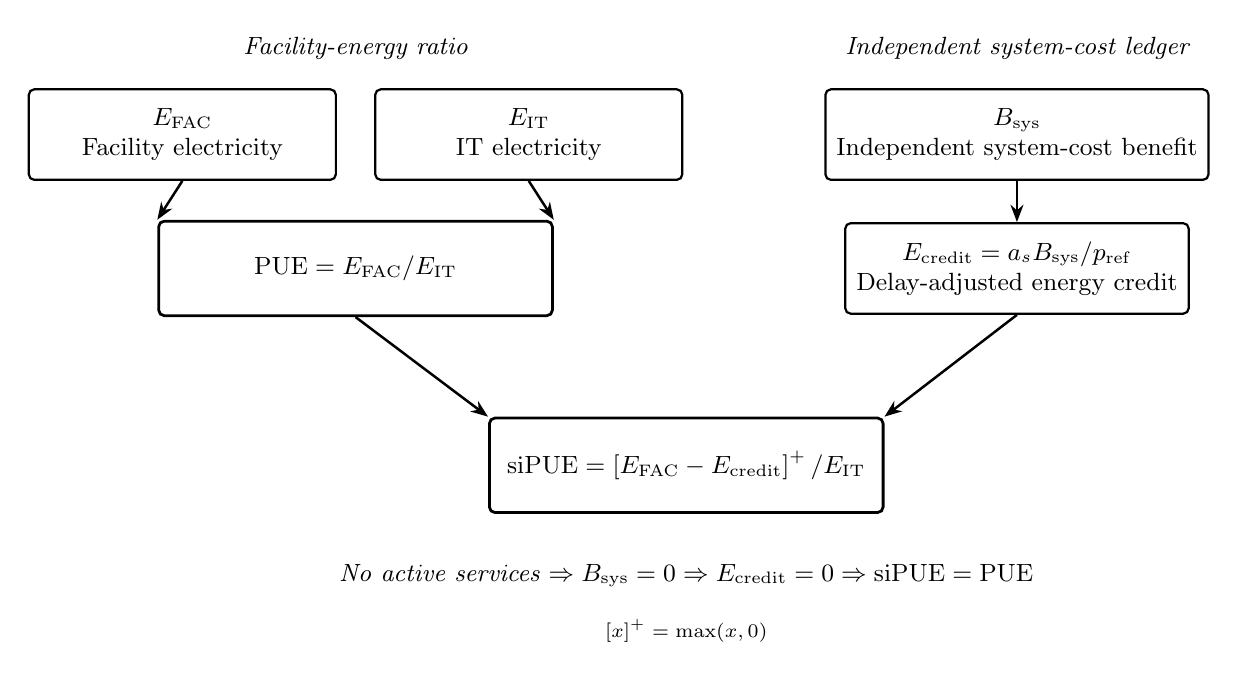
\begin{tikzpicture}[
    >=Stealth,
    node distance=9mm and 16mm,
    every node/.style={align=center},
    box/.style={
        rectangle,
        draw=black,
        rounded corners=2pt,
        minimum width=3.9cm,
        minimum height=1.15cm,
        line width=0.8pt,
        inner sep=4pt,
        font=\small
    },
    calc/.style={
        rectangle,
        draw=black,
        rounded corners=2pt,
        minimum width=5.0cm,
        minimum height=1.2cm,
        line width=1.0pt,
        inner sep=5pt,
        font=\small
    },
    header/.style={
        font=\itshape\small
    },
    flow/.style={
        -{Stealth[length=2.2mm]},
        line width=0.9pt
    }
]

%--- Left branch ---------------------------------------------------------------
\node[header] (hL) at (0,2.25) {Facility-energy ratio};

\node[box] (efac) at (-2.2,1.15)
    {$E_{\mathrm{FAC}}$\\Facility electricity};

\node[box] (eit) at (2.2,1.15)
    {$E_{\mathrm{IT}}$\\IT electricity};

\node[calc] (pue) at (0,-0.55)
    {$\mathrm{PUE}=E_{\mathrm{FAC}}/E_{\mathrm{IT}}$};

\draw[flow] (efac.south) -- (pue.north west);
\draw[flow] (eit.south)  -- (pue.north east);

%--- Right branch --------------------------------------------------------------
\node[header] (hR) at (8.4,2.25) {Independent system-cost ledger};

\node[box] (bsys) at (8.4,1.15)
    {$B_{\mathrm{sys}}$\\Independent system-cost benefit};

\node[box] (credit) at (8.4,-0.55)
    {$E_{\mathrm{credit}} = a_s B_{\mathrm{sys}}/p_{\mathrm{ref}}$\\Delay-adjusted energy credit};

\draw[flow] (bsys.south) -- (credit.north);

%--- Final metric --------------------------------------------------------------
\node[calc] (sipue) at (4.2,-3.05)
    {$\mathrm{siPUE}
      = \left[E_{\mathrm{FAC}} - E_{\mathrm{credit}}\right]^+/E_{\mathrm{IT}}$};

\draw[flow] (pue.south)    -- (sipue.north west);
\draw[flow] (credit.south) -- (sipue.north east);

%--- Annotation ----------------------------------------------------------------
\node[font=\itshape\small, align=center] at (4.2,-4.45)
    {No active services $\Rightarrow B_{\mathrm{sys}}=0
    \Rightarrow E_{\mathrm{credit}}=0
    \Rightarrow \mathrm{siPUE}=\mathrm{PUE}$};

\node[font=\scriptsize] at (4.2,-5.15)
    {$[x]^+ = \max(x,0)$};

\end{tikzpicture}
}
\caption{Metric logic for siPUE. PUE is the internal facility-energy ratio computed from measured electricity only. siPUE subtracts a delay-adjusted, energy-equivalent credit associated with the independent system-cost benefit from the facility-energy term before normalizing by IT electricity. The positive-part operator ensures that the adjusted numerator cannot become negative. When no services are active, $E_{\mathrm{credit}}=0$ and $\mathrm{siPUE}=\mathrm{PUE}$.}
\label{fig:sipue-metric-story}
\end{figure}




\subsection{Definition and interpretation of siPUE}

siPUE treats the data center as both a consumer and a prosumer of the local energy system. It reports both roles in one energy-equivalent number; Figure~\ref{fig:sipue-metric-story} summarizes the resulting metric logic. PUE captures the consumer role through the electricity drawn to serve the IT load. The credit term captures the prosumer role through heat recovery, flexibility, peak relief, and avoided carbon damage provided to the system. This second role is priced through the independent system-cost ledger defined below (Table~\ref{tab:sipue-boundary}), so the prosumer credit reflects value delivered to the system. Private cash flow from the same prosumer activity (heat and flexibility revenue, capex, land, financing) is tracked separately in the lifecycle market-cost objective (Table~\ref{tab:sipue-boundary}).

PUE is defined as
\begin{equation}
\text{PUE} = \frac{E_{\text{FAC}}}{E_{\text{IT}}},
\end{equation}
where $E_{\text{FAC}}$ is modeled facility electricity and $E_{\text{IT}}$ is delivered IT electricity. siPUE keeps this denominator and adjusts the numerator by a system-benefit credit. Let superscript $0$ denote the services-disabled comparator and $d$ a service-active design. The independent system-cost ledger is
\begin{equation}
C_{\text{ind}}^d =
C_{\text{el}}^d
+ C_{\text{trans}}^d
+ C_{\text{peak}}^d
+ C_{\text{CO2,dam}}^d
- V_{\text{heat}}^d
- V_{\text{flex}}^d,
\label{eq:independent-cost-ledger}
\end{equation}
where $C_{\text{el}}$, $C_{\text{trans}}$, $C_{\text{peak}}$, and $C_{\text{CO2,dam}}$ are electricity-resource, network, peak-capacity, and carbon-damage costs, and $V_{\text{heat}}$ and $V_{\text{flex}}$ are avoided heat and flexibility costs. $V_{\text{heat}}$ includes only avoided boiler fuel cost and avoided variable O\&M; it excludes any carbon or emissions term. $V_{\text{flex}}$ is a fixed avoided reserve-capacity value, independent of carbon pricing. The carbon-damage value of the emissions avoided by displacing boiler heat or thermal generation is credited separately through $C_{\text{CO2,dam}}$. This term draws on the same physical emissions ledger used for $V_{\text{heat}}$'s displaced fuel but applies a separate cost basis: social carbon cost times avoided tCO2. The credited system benefit is
\begin{equation}
B_{\text{sys}}^d =
C_{\text{ind}}^0 - C_{\text{ind}}^d.
\label{eq:system-benefit}
\end{equation}
Positive terms in $B_{\text{sys}}$ are avoided independent system costs; negative terms are additional system burdens. Components are aggregated before any clipping, so a design with negative net system benefit receives a negative credit and siPUE rises relative to PUE.

\begin{table}[tbp]
\centering
\small
\caption{Accounting boundary for the siPUE system-benefit term (upper panel) and treatment of the three carbon mechanisms (lower panel).}
\label{tab:sipue-boundary}
\begin{tabularx}{\linewidth}{X X}
\toprule
Included in $B_{\text{sys}}$ & Excluded from $B_{\text{sys}}$ \\
\midrule
Electricity resource-cost changes, transmission or network-cost changes, independent peak-capacity effects, carbon-damage changes, avoided heat-system cost, and avoided flexibility-system cost. & Private heat and flexibility revenues, IT service revenue, ETS or carbon-market payments, capex, land lease or opportunity cost, private demand charges, taxes, subsidies, and financing terms. \\
\bottomrule
\end{tabularx}

\vspace{2mm}
\begin{tabularx}{\linewidth}{L{2.6cm} X L{1.9cm} L{2.1cm}}
\toprule
Carbon mechanism & Purpose & In optimization? & In siPUE credit? \\
\midrule
ETS payment & Private compliance and dispatch cost in the market ledger. & Yes & No \\
Carbon-damage value & External damage value in the independent accounting ledger. & Ledger only & Yes \\
Physical carbon cap & Row-level planning constraint shared by the services-disabled comparator, baseline, robust, and scenario-perfect modes. & Yes & No direct monetary credit \\
\bottomrule
\end{tabularx}
\end{table}

Heat and flexibility revenues remain in the market objective, while carbon damage enters only the independent system ledger. ETS payments and carbon damage use the same emissions data but different prices, so emissions are not counted twice.

All quantities entering Eqs.~(\ref{eq:independent-cost-ledger})--(\ref{eq:system-benefit}) are annual and undiscounted: $E_{\text{FAC}}$ and $E_{\text{IT}}$ are expressed in MWh per representative modeled operating year, whereas $C_{\text{ind}}$ and $B_{\text{sys}}$ are expressed in EUR per year for that same year.

The delay-adjusted energy credit is
\begin{equation}
E_{\text{credit}} =
a_s \frac{B_{\text{sys}}}{p_{\text{ref}}},
\label{eq:sipue-credit}
\end{equation}
where $p_{\text{ref}}$ is a fixed unit-conversion price in EUR/MWh and $a_s \in [0,1]$ is the dimensionless lifecycle availability factor after construction delay. In the canonical run, $p_{\text{ref}}=56.63$~EUR/MWh, the electricity-resource marginal cost at the data-center node in the identity solve. The identity solve sets both efficiency investment and service capacity to zero, so its marginal price cannot be shifted by the design choices siPUE evaluates. Anchoring $p_{\text{ref}}$ to the services-disabled comparator would allow its locked efficiency retrofit and carbon-cap treatment to influence a conversion factor common to every case. ETS payments and carbon damage are excluded from $p_{\text{ref}}$ because they are handled in separate ledgers.

$B_{\mathrm{sys}}$ is defined on an annual basis, whereas $a_s$ accounts for construction delay over the asset life. For post-construction siPUE, $a_s=1$; this form is used for annual reporting. Delay-adjusted siPUE retains $a_s$ and is used for investment decision making.
siPUE is
\begin{equation}
\text{siPUE} =
\frac{\left[E_{\text{FAC}} - E_{\text{credit}}\right]^+}{E_{\text{IT}}},
\label{eq:sipue}
\end{equation}
with $[z]^+=\max(0,z)$. Internal property checks verify nonnegativity, reduction to PUE when no services are active, delay behavior, carbon-ledger separation, scenario count, scale normalization, benefit monotonicity, and reference-price monotonicity.

The positive-part operator in Eq.~(\ref{eq:sipue}) is a safeguard that becomes active if the credited system value exceeds total facility electricity. Reported siPUE values remain well above zero. The smallest value is 0.96 under the low-conversion-price sensitivity (Table~\ref{tab:pref-sensitivity}), so the guard remains slack in the canonical results and siPUE remains a smooth function of $B_{\text{sys}}$. A value below one remains possible when the conversion price is low enough (Section~\ref{sec:pref-sensitivity}). In ledger terms, credited system value can exceed facility electricity in energy-equivalent terms. The site then yields a net benefit on the independent ledger while still consuming more electricity than its IT load. Because siPUE is a ledger indicator, the reference price must be reported alongside the physical PUE value.

siPUE also rewards integration that generates system value efficiently. A design with twice the installed service capacity of another can score worse if the additional capacity delivers less system value per unit of facility electricity consumed. This behavior is intentional: additional equipment improves the score only when its system value is large enough relative to its own electricity burden. Section~\ref{sec:results} shows this property in the reported designs: the robust design delivers roughly twice the absolute system benefit of the baseline design but still has a marginally higher (worse) siPUE.

\subsection{Reference-price sensitivity}
\label{sec:pref-sensitivity}

The reference price is the key conversion parameter in siPUE. Holding design and operation fixed, a multiplier $k$ gives
\begin{equation}
\text{siPUE}(k) =
\frac{\left[E_{\text{FAC}} - a_s B_{\text{sys}} /(k p_{\text{ref}})\right]^+}{E_{\text{IT}}}.
\label{eq:sipue-pref-sensitivity}
\end{equation}

$p_{\text{ref}}$ is held constant across designs and uncertainty states. Table~\ref{tab:pref-sensitivity} varies only the conversion factor in Eq.~(\ref{eq:sipue-pref-sensitivity}); dispatch, heat delivery, emissions, PUE, and $B_{\text{sys}}$ remain unchanged.

\begin{table}[tbp]
\centering
\small
\caption{Reference-price sensitivity for the canonical robust rows. Dispatch and ledgers are held fixed; only the value-to-energy conversion factor changes. Average siPUE uses IT-energy weights across archetypes.}
\label{tab:pref-sensitivity}
\begin{tabularx}{\linewidth}{L{3.0cm} Y r}
\toprule
Reference-price case & Interpretation & Average siPUE \\
\midrule
$0.5p_{\text{ref}}$ & Low conversion price; stronger energy credit & 0.96 \\
$1.0p_{\text{ref}}$ & Canonical frozen reference price & 1.15 \\
$1.5p_{\text{ref}}$ & High conversion price; weaker energy credit & 1.21 \\
\bottomrule
\end{tabularx}
\end{table}

The sensitivity shows that $p_{\text{ref}}$ scales the magnitude of the credit even when every physical and monetary ledger is unchanged. With $p_{\text{ref}}>0$ and $a_s\ge0$, the sign of $E_{\text{credit}}$ follows the sign of $B_{\text{sys}}$ for any conversion price. Changing $p_{\text{ref}}$ therefore preserves whether siPUE lies above or below PUE and scales only the size of the gap. The conversion price is a disclosed reporting convention. siPUE should be reported with the reference-price rule and a sensitivity band.

\subsection{Reporting protocol and computability}
\label{sec:reporting-protocol}

siPUE requires more than facility meter readings. While PUE requires only facility and IT electricity measurements, siPUE also requires a standardized no-services reference case, avoided-cost values for the surrounding energy system, and a carbon-damage value. These inputs lie outside the facility boundary, which places siPUE in a different reporting class from PUE, ERF, CUE, or REF.

The operator can measure the physical quantities: facility and IT electricity, delivered heat $H^{\text{sold}}$, contracted and delivered reserve, peak import, and installed service capacity. System-side values must be supplied by the network or heat-system operator or specified by the regulator as published defaults. These values include avoided heat-system and reserve-capacity unit values, peak-capacity and network unit costs, the reference price $p_{\text{ref}}$, and the social cost of carbon. siPUE is therefore a jointly verified indicator, computed from operator-metered physical quantities and externally published unit values, and it should be reported alongside those unit values.

The no-services reference case is fixed by convention: service capacities are set to zero while the efficiency retrofit and other physical parameters remain at their as-built values. A facility with no service capacity is therefore its own comparator and reports $\text{siPUE}=\text{PUE}$.

\subsection{Two-stage design model}

Let $s \in \mathcal{S}$ index the shared uncertainty states, $x$ denote design variables, and $y_s$ denote hourly operational variables. Stage~1 solves a scenario-perfect benchmark:
\begin{equation}
C_s^{\star} = \min_{x,y_s} C_s(x,y_s),
\label{eq:stage-one}
\end{equation}
where $C_s$ is lifecycle market cost. Stage~2 chooses one shared design $\hat{x}$ per archetype using min-max regret \cite{savage1951theory,MR-1626-RPC}. All ten states receive equal weight, and each archetype is solved independently. Regret is normalized by each scenario's present-value-discounted lifetime IT energy $E_{\text{IT},s}^{\text{PV}}$:
\begin{equation}
R_s(\hat{x}) =
\frac{C_s(\hat{x},y_s)-C_s^{\star}}{\max(\epsilon, E_{\text{IT},s}^{\text{PV}})}.
\label{eq:normalised-regret}
\end{equation}
The robust design minimizes $Z=\max_{s\in\mathcal{S}}R_s(\hat{x})$ directly for each archetype. Table~\ref{tab:solve-modes} lists the five solve modes and states which of them are reported as design cases.

The canonical run sets the efficiency reduction to 0.15 in the services-disabled comparator, baseline, robust, and scenario-perfect cases. The optimized capacity variables include heat-exchanger capacity, heat-pump capacity, flexibility capacity, battery energy and power capacity, and associated land use. The identity solve keeps service capacity and efficiency reduction at zero. As a fairness check, the services-disabled comparator was re-solved in all 40 canonical rows with efficiency chosen freely from the same discrete candidate set (0\% or 15\%). The 15\% retrofit was selected in every row, indicating that the comparator's unconstrained economics favor the retrofit independently of any service. Thus, the locked value matches the freely optimized choice.

\begin{table}[tbp]
\centering
\scriptsize
\setlength{\tabcolsep}{3pt}
\caption{Solve modes used in the study and the role of each. ``Reported as a
design case'' identifies the modes whose PUE and siPUE values appear in the
results.}
\label{tab:solve-modes}
\begin{tabularx}{\linewidth}{L{2.5cm} L{4.0cm} L{1.9cm} Y}
\toprule
Solve mode & Definition & Reported as a design case? & Quantity it supplies \\
\midrule

Identity
& No services and no efficiency investment.
& No
& Checks that $\text{siPUE}=\text{PUE}$ and sets the reference price
$p_{\text{ref}}$. \\

Services-disabled comparator
& No services; the 15\% efficiency retrofit and all physical constraints are retained.
& Yes (reference case)
& Provides the reference ledger $C_{\text{ind}}^{0}$ in
Eq.~(\ref{eq:system-benefit}) and the carbon-cap basis in
Eq.~(\ref{eq:carbon-cap-floor}). \\

Baseline
& Assumed baseline service-active portfolio
(Table~\ref{tab:design-capacities}).
& Yes
& Provides baseline PUE, siPUE, and system benefit. \\

Robust
& One shared min--max-regret design per archetype across the ten states.
& Yes
& Provides robust PUE, siPUE, system benefit, and credit decomposition. \\

Scenario-perfect
& Best design for each individual scenario.
& No
& Provides the benchmark $C_s^{\star}$ in
Eq.~(\ref{eq:normalised-regret}). KPIs are omitted because this benchmark produces
one design per scenario. \\

\bottomrule
\end{tabularx}
\end{table}


\subsection{Operational constraints and ledgers}

Hourly operation is a linear program. The facility balance links grid import, battery operation, IT load, cooling, and heat-pump electricity. Heat export is bounded by heat-exchanger and heat-pump capacity, recoverable heat, pipe limits, and district-heating acceptance. Flexibility is modeled as reserve availability; routine activation is outside the settlement basis \cite{Takci2025,Crozier2025}. Deliverability is enforced through IT-load headroom, controllable capacity, unused battery inverter capacity, stored energy above the UPS reserve, and parasitic overhead.

The electricity system is a stylized three-node DC-OPF with thermal generation, renewable availability, line capacities, and nodal settlement prices (Figure~\ref{fig:nodal-power}). Carbon costs follow the market/independent ledger split in Table~\ref{tab:sipue-boundary}. Land is represented as lease or opportunity cost tied to core facility, cooling, heat, flexibility, and battery footprints. The heat system is represented as a heat-recovery chain with storage and sales across price segments (Figure~\ref{fig:nodal-heat}).

\begin{figure}[tbp]
\centering
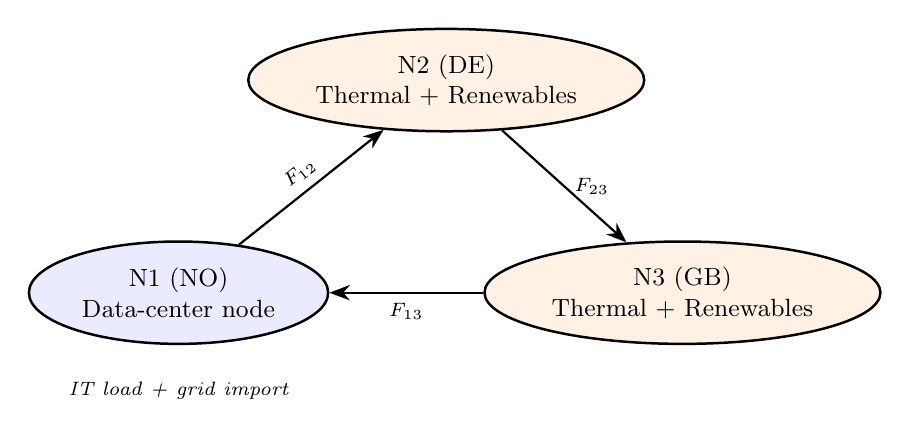
\begin{tikzpicture}[
node/.style={draw, ellipse, minimum width=2.9cm, minimum height=1.3cm, align=center, font=\small, line width=0.9pt},
flowarrow/.style={-{Stealth[length=2.6mm]}, thick}
]
\node[node, fill=blue!8] (n1) at (0,0) {N1 (NO)\\Data-center node};
\node[node, fill=orange!10] (n2) at (3.4,2.7) {N2 (DE)\\Thermal + Renewables};
\node[node, fill=orange!10] (n3) at (6.4,0) {N3 (GB)\\Thermal + Renewables};

\draw[flowarrow] (n1) -- node[above, sloped, font=\scriptsize] {$F_{12}$} (n2);
\draw[flowarrow] (n2) -- node[right, font=\scriptsize] {$F_{23}$} (n3);
\draw[flowarrow] (n3) -- node[below, sloped, font=\scriptsize] {$F_{13}$} (n1);

\node[below=0.35cm of n1, font=\scriptsize\itshape, align=center] {IT load + grid import};
\end{tikzpicture}
\caption{Stylized three-node DC-OPF electricity network. Each node represents one modeled country group, N1 (Nordics: Norway, Sweden, Denmark, Finland, Iceland), N2 (Central Europe: Germany, Belgium, Netherlands, France), and N3 (United Kingdom); one representative country is shown per node. $F_{12}$, $F_{23}$, and $F_{13}$ are the linearized DC power flows between node pairs; arrow direction is illustrative, since flows are signed variables that can reverse hour to hour. The data-center node shown here (N1) is illustrative. Each archetype's own scenario location determines which node it actually attaches to. Thermal generation capacity is 5,500~MW at each node. Calibrated baseline line capacities, before the per-scenario congestion multiplier (Table~\ref{tab:uncertainty-state-multipliers}), are 938.3~MW ($F_{12}$), 422.6~MW ($F_{23}$), and 1345.3~MW ($F_{13}$); see Table~\ref{tab:parameters} (Appendix A.10) for the full network parameter list.}
\label{fig:nodal-power}
\end{figure}

\begin{figure}[tbp]
\centering
\resizebox{\linewidth}{!}{%
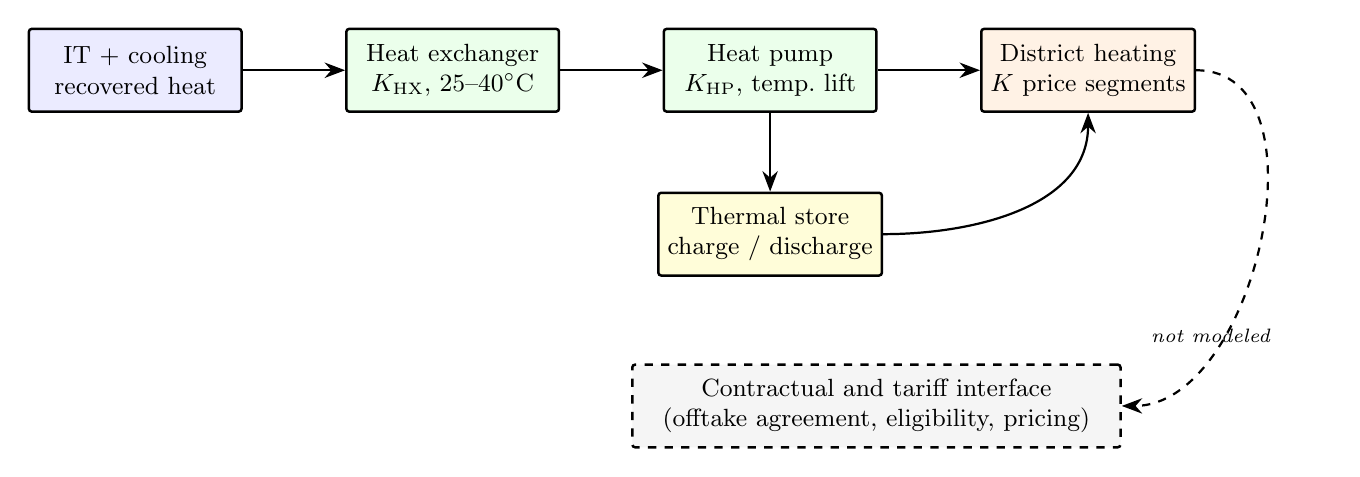
\begin{tikzpicture}[
box/.style={draw, rectangle, rounded corners=1pt, align=center, minimum width=2.7cm, minimum height=1.05cm, font=\small, line width=0.9pt},
flowarrow/.style={-{Stealth[length=2.6mm]}, thick}
]
\node[box, fill=blue!8] (src) at (0,0) {IT + cooling\\recovered heat};
\node[box, fill=green!8, right=1.3cm of src] (hx) {Heat exchanger\\$K_{\text{HX}}$, 25--40$^\circ$C};
\node[box, fill=green!8, right=1.3cm of hx] (hp) {Heat pump\\$K_{\text{HP}}$, temp.\ lift};
\node[box, fill=orange!10, right=1.3cm of hp] (dh) {District heating\\$K$ price segments};
\node[box, fill=yellow!15, below=1.0cm of hp] (store) {Thermal store\\charge / discharge};

\draw[flowarrow] (src) -- (hx);
\draw[flowarrow] (hx) -- (hp);
\draw[flowarrow] (hp) -- (dh);
\draw[flowarrow] (hp.south) -- (store.north);
\draw[flowarrow] (store.east) to[out=0,in=270] (dh.south);

% --- Contractual tier: outside the modeled physical chain ---
\node[box, fill=gray!8, dashed, minimum width=6.2cm, below=1.1cm of store, xshift=1.35cm]
  (contract) {Contractual and tariff interface\\(offtake agreement, eligibility, pricing)};
\draw[flowarrow, dashed] (dh.east) to[out=0,in=0] (contract.east);

\node[font=\scriptsize\itshape, align=left, right=0.25cm of contract.north east, yshift=0.35cm]
  {not modeled};
\end{tikzpicture}
}
\caption{Heat-recovery chain as modeled, with the commercial interface that determines whether the chain is investable. Recovered heat from IT and cooling loads passes through the heat exchanger and heat pump to become delivered heat, is optionally buffered in a thermal store, and is sold into up to $K$ district-heating price segments. The solid boxes are the physical and price-segment representation inside the optimization model. The dashed box is the contractual and tariff interface (Section~\ref{sec:policy-context}): a design can satisfy every technical requirement and still fail commercially if the offtake contract is missing, but this interface is exogenous to the model and enters only through the district-heating price and acceptance capacity.}
\label{fig:nodal-heat}
\end{figure}

\subsection{Data and scenario design}

Figure~\ref{fig:model-pipeline} summarizes the workflow from inputs to reported metrics. The model uses a calibrated 8,760-hour, three-node time series compressed into seven representative days. Stratified medoid clustering selects representative days from seasonal strata using standardized fuel-price, load, renewable, net-load, calendar, ambient-temperature, and district-heating features. Cluster weights preserve annual hours. Fixed annual terms enter once outside the representative-day weighting. The seven days are concatenated into one operating horizon. Battery state of charge and peak import are evaluated across the combined sample, with state carried across day boundaries.
\begin{figure}[tbp]
\centering
\footnotesize
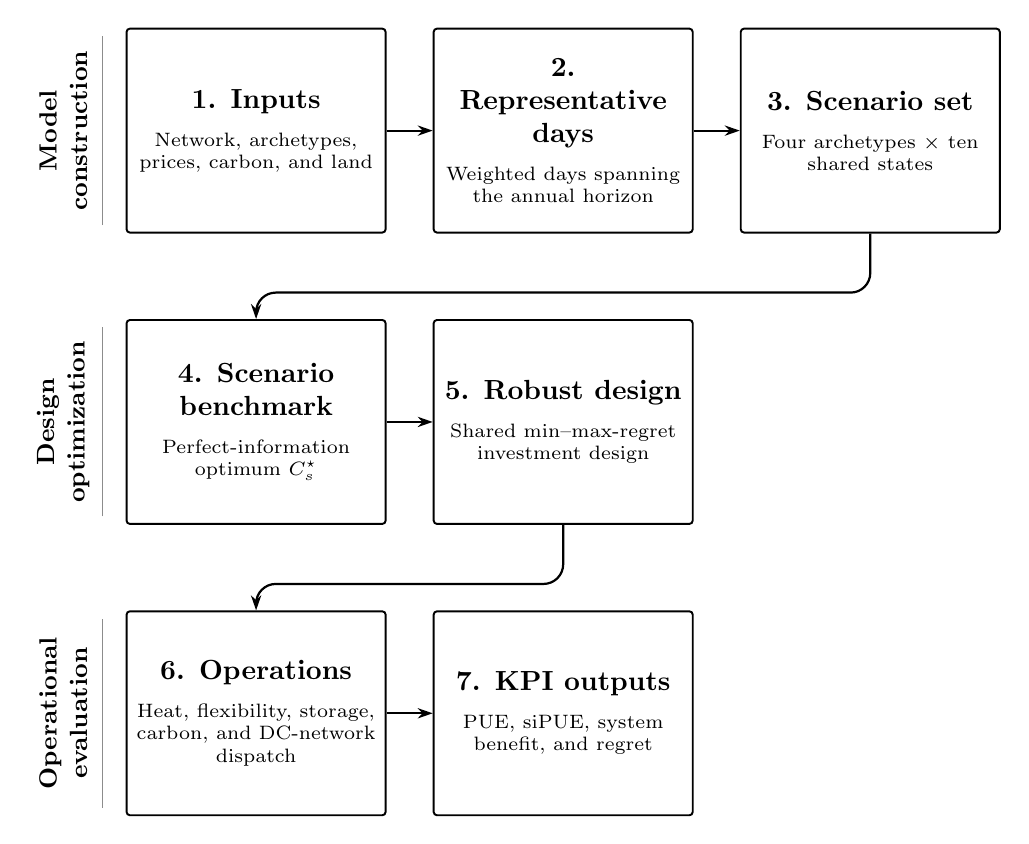
\begin{tikzpicture}[
    stage/.style={
        rectangle,
        draw=black,
        rounded corners=1.2pt,
        inner sep=1.2mm,
        line width=0.7pt,
        align=center
    },
    phase/.style={
        font=\bfseries\small,
        align=center
    },
    phaserule/.style={
        line width=0.6pt
    },
    flow/.style={
        -{Stealth[length=1.9mm,width=1.3mm]},
        line width=0.8pt
    }
]

%--- Row 1: Model construction ------------------------------------------------
\node[stage] (s1) at (0.00,5.00) {\stagecontent{1. Inputs}{Network, archetypes, prices, carbon, and land}};
\node[stage] (s2) at (3.90,5.00) {\stagecontent{2. Representative days}{Weighted days spanning the annual horizon}};
\node[stage] (s3) at (7.80,5.00) {\stagecontent{3. Scenario set}{Four archetypes $\times$ ten shared states}};

\draw[flow] (s1.east) -- (s2.west);
\draw[flow] (s2.east) -- (s3.west);

%--- Row 2: Design optimization ----------------------------------------------
\node[stage] (s4) at (0.00,1.30) {\stagecontent{4. Scenario benchmark}{Perfect-information optimum $C_s^{\star}$}};
\node[stage] (s5) at (3.90,1.30) {\stagecontent{5. Robust design}{Shared min--max-regret investment design}};

\draw[flow] (s4.east) -- (s5.west);

%--- Row 3: Operational evaluation -------------------------------------------
\node[stage] (s6) at (0.00,-2.40) {\stagecontent{6. Operations}{Heat, flexibility, storage, carbon, and DC-network dispatch}};
\node[stage] (s7) at (3.90,-2.40) {\stagecontent{7. KPI outputs}{PUE, siPUE, system benefit, and regret}};

\draw[flow] (s6.east) -- (s7.west);

%--- Row wraps: end of one row to the start of the next ----------------------
\draw[flow, rounded corners=2.5mm]
    (s3.south) -- ++(0,-0.75) -| (s4.north);
\draw[flow, rounded corners=2.5mm]
    (s5.south) -- ++(0,-0.75) -| (s6.north);

%--- Phase labels as left-hand row headers ----------------------------------
\node[phase, rotate=90, anchor=center] at (-2.45, 5.00) {Model\\construction};
\node[phase, rotate=90, anchor=center] at (-2.45, 1.30) {Design\\optimization};
\node[phase, rotate=90, anchor=center] at (-2.45,-2.40) {Operational\\evaluation};

\draw[phaserule, draw=black!45] (-1.95, 3.80) -- (-1.95, 6.20);
\draw[phaserule, draw=black!45] (-1.95, 0.10) -- (-1.95, 2.50);
\draw[phaserule, draw=black!45] (-1.95,-3.60) -- (-1.95,-1.20);

\end{tikzpicture}

\caption{Model workflow from input construction to performance evaluation. Each
phase proceeds from left to right; the elbow arrows wrap from the end of one phase to the
start of the next. Inputs are reduced to weighted representative days and combined
with the shared scenario set. Scenario-specific perfect-information benchmarks
$C_s^{\star}$ are used to formulate the shared min--max-regret design, which is then
evaluated using the operational model and reported through energy, system-benefit,
and regret metrics.}
\label{fig:model-pipeline}

\end{figure}

The canonical scenario set comprises four archetypes (AI/HPC, Hyperscale cloud, Colocation, and Enterprise/edge), each evaluated under ten shared uncertainty states, for a total of 40 rows. Each row is solved in every mode listed in Table~\ref{tab:solve-modes}. States vary service prices, heat conditions, construction delay, carbon caps, and operating conditions. Table~\ref{tab:archetypes} defines the four archetypes. Archetype base recoverable-heat fractions are 0.20--0.50 \cite{11,Hao2025}; state multipliers raise effective LP inputs to 0.17--0.58 in the canonical rows. Outputs are normalized by IT energy or IT capacity where appropriate, and every IT-weighted mean reported below uses the annual IT energies in Table~\ref{tab:archetypes} as weights.

\begin{table}[tbp]
\centering
\scriptsize
\setlength{\tabcolsep}{4pt}
\caption{Archetype definitions. Annual IT energy is the weight used in every IT-energy-weighted mean reported in Section~\ref{sec:results}. $\phi$ is the flexible-load fraction (Appendix A.3) and $\alpha^{\text{base}}$ the base cooling-overhead ratio before the efficiency retrofit (Appendix A.1). District-heating acceptance capacity is driven by the shared uncertainty state's heat demand (Table~\ref{tab:uncertainty-state-levels}), not by archetype technology, so the reported figure is the same state-driven quantity for every archetype (mean 19.3~MW$_{\text{th}}$; range 10.0--33.9~MW$_{\text{th}}$ across the ten states); each archetype's own heat-exchanger capacity and recoverable-heat fraction then determine how much of that shared capacity it can actually use.}
\label{tab:archetypes}
\begin{tabular}{l r r r r r r}
\toprule
Archetype & IT capacity & Annual IT energy & $\alpha^{\text{base}}$ & $\phi$ & Recoverable-heat & DH acceptance \\
 & (MW) & (GWh/year) & (--) & (--) & fraction (--) & capacity (MW$_{\text{th}}$) \\
\midrule
AI/HPC            & 40.0 & 345.0 & 0.12 & 0.24 & 0.50 & 19.3 \\
Hyperscale cloud  & 60.0 & 515.1 & 0.18 & 0.16 & 0.45 & 19.3 \\
Colocation        & 25.0 & 189.5 & 0.30 & 0.10 & 0.32 & 19.3 \\
Enterprise/edge   & 8.0  & 61.5  & 0.42 & 0.05 & 0.20 & 19.3 \\
\bottomrule
\end{tabular}
\end{table}

Table~\ref{tab:uncertainty-state-levels} and Table~\ref{tab:uncertainty-state-multipliers} report the ten shared uncertainty states in full; the scenario generator and seed are available with the released code (Code availability, below).

\begin{table}[tbp]
\centering
\tiny
\setlength{\tabcolsep}{1.5pt}
\caption{Shared uncertainty states, absolute input levels. El. price and heat price are EUR/MWh(th); flex price is EUR/MW-h; ETS and carbon-damage prices are EUR/tCO2; delay is months.}
\label{tab:uncertainty-state-levels}
\begin{tabular}{l l r r r r r r r r}
\toprule
State & Loc. & El. price & El. vol. & Heat price & Heat dem. & Flex price & ETS & Damage & Delay \\
\midrule
1 Central-base & Netherlands & 65 & 18 & 58 & 50 & 18 & 65 & 120 & 6 \\
2 Clean-cool & Norway & 48 & 13 & 48 & 62 & 16 & 45 & 80 & 0 \\
3 High-ETS & Germany & 72 & 24 & 62 & 48 & 21 & 105 & 160 & 6 \\
4 Heat-rich & Denmark & 58 & 20 & 78 & 78 & 20 & 75 & 140 & 0 \\
5 Flex-rich & UK & 82 & 30 & 52 & 30 & 31 & 80 & 130 & 12 \\
6 Cooling-stress & France & 70 & 22 & 55 & 38 & 18 & 70 & 110 & 6 \\
7 Congestion-stress & Belgium & 76 & 27 & 60 & 44 & 24 & 85 & 180 & 6 \\
8 Storage-limited & Sweden & 54 & 19 & 50 & 55 & 17 & 60 & 100 & 0 \\
9 Cost-stress & Netherlands & 74 & 25 & 56 & 42 & 19 & 90 & 200 & 12 \\
10 Service-upside & Denmark & 60 & 21 & 82 & 70 & 29 & 75 & 150 & 6 \\
\bottomrule
\end{tabular}
\end{table}

\begin{table}[tbp]
\centering
\tiny
\setlength{\tabcolsep}{2.5pt}
\caption{Shared uncertainty states, multipliers applied to archetype base values. Cong. = congestion, Cool. OH = cooling overhead, Free cool. = free-cooling availability, Heat rec. = heat-recovery fraction, HP COP = heat-pump coefficient of performance, Flex avail. = flexibility availability, Storage = storage availability, Capex and Land are cost multipliers.}
\label{tab:uncertainty-state-multipliers}
\begin{tabular}{l r r r r r r r r r}
\toprule
State & Cong. & Cool. OH & Free cool. & Heat rec. & HP COP & Flex avail. & Storage & Capex & Land \\
\midrule
1 Central-base & 1.00 & 1.00 & 1.00 & 1.00 & 1.00 & 1.00 & 1.00 & 1.00 & 1.00 \\
2 Clean-cool & 1.20 & 0.82 & 1.25 & 1.10 & 1.08 & 0.95 & 1.10 & 0.90 & 0.80 \\
3 High-ETS & 0.90 & 1.05 & 0.95 & 0.95 & 0.95 & 0.90 & 0.90 & 1.00 & 1.10 \\
4 Heat-rich & 0.85 & 0.92 & 1.15 & 1.15 & 1.05 & 1.00 & 1.00 & 1.05 & 0.95 \\
5 Flex-rich & 0.75 & 1.08 & 0.90 & 0.90 & 0.90 & 1.20 & 1.00 & 1.00 & 1.05 \\
6 Cooling-stress & 1.05 & 1.28 & 0.70 & 0.85 & 0.92 & 0.90 & 0.90 & 1.10 & 1.00 \\
7 Congestion-stress & 0.60 & 1.12 & 0.90 & 1.00 & 0.95 & 1.05 & 0.90 & 1.05 & 1.10 \\
8 Storage-limited & 1.10 & 0.88 & 1.20 & 1.05 & 1.05 & 0.95 & 0.35 & 1.00 & 0.90 \\
9 Cost-stress & 0.80 & 1.15 & 0.85 & 0.90 & 0.90 & 0.90 & 0.80 & 1.35 & 1.30 \\
10 Service-upside & 0.95 & 0.95 & 1.10 & 1.15 & 1.08 & 1.15 & 1.15 & 0.90 & 0.95 \\
\bottomrule
\end{tabular}
\end{table}

\section{Results and Discussion}
\label{sec:results}

The PUE--siPUE split is reported first, followed by credit decomposition, robustness checks, sensitivity analysis, and a face-validity assessment \cite{UptimeInstitute2024Survey,EUSmartCities2024Mantsala}.

\subsection{PUE and siPUE move differently}

Across the canonical study, the two metrics move in opposite directions for the same designs in most rows. Every service-active row raises PUE: all 40 baseline rows and all 40 robust rows show higher PUE than the services-disabled comparator. siPUE moves the other way in 36 of the 40 baseline rows and in 23 of the 40 robust rows, yielding a more even split. Figures~\ref{fig:kpi-pue} and~\ref{fig:kpi-sipue} show this by archetype. PUE rises with integration intensity in every case, while siPUE remains unchanged or falls for the same designs.

\begin{figure}[tbp]
\centering
\includegraphics[width=0.85\linewidth]{final_06_kpi_pue.pdf}
\caption{PUE by archetype across the reported design cases and the identity solve, with the IT-weighted mean shown dashed. The identity solve is included to show the metric identity: at that point, PUE here and siPUE in Figure~\ref{fig:kpi-sipue} take the same value by construction; it is not a design case (Table~\ref{tab:solve-modes}).}
\label{fig:kpi-pue}
\end{figure}

\begin{figure}[tbp]
\centering
\includegraphics[width=0.85\linewidth]{final_07_kpi_sipue.pdf}
\caption{siPUE by archetype across the reported design cases and the identity solve, with the IT-weighted mean shown dashed. The same jointly optimized designs that push PUE up across every archetype (Figure~\ref{fig:kpi-pue}) leave siPUE flat or falling here, because siPUE credits the independent system-cost benefit omitted by PUE.}
\label{fig:kpi-sipue}
\end{figure}

Table~\ref{tab:kpi-summary} reports the canonical averages behind this split, weighted by each archetype's annual IT energy (Table~\ref{tab:archetypes}). The \emph{facility-energy burden} of a design is its PUE increase over the comparator, $\Delta\text{PUE}=\text{PUE}^d-\text{PUE}^0$, and the \emph{credit} is the PUE-to-siPUE gap, $E_{\text{credit}}/E_{\text{IT}}=\text{PUE}^d-\text{siPUE}^d$; their ratio measures the energy-equivalent system value associated with each additional unit of facility electricity.

The services-disabled comparator is the reference case: it carries the same efficiency retrofit and carbon-cap treatment as the service-active cases and gives PUE and siPUE values of 1.17. Against it, the baseline design raises average PUE to 1.24 while lowering average siPUE to 1.14, delivering 5.60~EUR/MWh IT of delay-adjusted system benefit, about 10\% of the reference electricity price and a credit about 1.40 times its facility-energy burden. The robust design raises PUE further, to 1.34, and lowers siPUE to 1.15, delivering a larger absolute benefit, 10.56~EUR/MWh IT, about 19\% of the reference price, with a smaller credit-to-burden ratio of about 1.10. The baseline design therefore has a marginally lower average siPUE, whereas the robust design creates more absolute system value at a lower benefit-to-burden ratio. This pattern is consistent with diminishing marginal system value as integration intensity increases and with the non-monotonicity property noted in Section~\ref{sec:methodology}.

\begin{table}[tbp]
\centering
\scriptsize
\setlength{\tabcolsep}{3pt}
\caption{Compact metric benchmark across the 40 canonical rows, weighted by each archetype's annual IT energy. Carbon, heat, and emissions are kept as separate ledgers with their own labels. Differences and ratios quoted in the text are computed from unrounded values and then rounded, so they need not equal the difference of the two-decimal entries shown here; for example the unrounded robust burden is $+0.18$, while the rounded PUE column implies $+0.17$.}
\label{tab:kpi-summary}
\begin{tabularx}{\linewidth}{L{3.05cm} >{\raggedleft\arraybackslash}X >{\raggedleft\arraybackslash}X >{\raggedleft\arraybackslash}X >{\raggedleft\arraybackslash}X >{\raggedleft\arraybackslash}X}
\toprule
Design case & PUE & Delay-adj. siPUE & Post-constr. siPUE & System benefit (EUR/MWh IT) & Benefit excl. carbon (EUR/MWh IT) \\
\midrule
Services-disabled comparator & 1.17 & 1.17 & 1.17 & 0.00 & 0.00 \\
Baseline & 1.24 & 1.14 & 1.13 & 5.60 & 3.43 \\
Robust & 1.34 & 1.15 & 1.14 & 10.56 & 5.10 \\
\bottomrule
\end{tabularx}
\end{table}

These changes are unevenly distributed across archetypes, and the ranking changes between the two service-active cases. Hyperscale cloud earns the largest baseline benefit (6.38~EUR/MWh IT), consistent with its larger baseline heat-exchanger and flexibility capacity (Table~\ref{tab:design-capacities}), but shows the smallest absolute increase under the robust design (to 9.30~EUR/MWh IT). Colocation and Enterprise/edge begin with lower benefits (4.61 and 2.35~EUR/MWh IT) but more than double under the robust design (to 12.91 and 9.76~EUR/MWh IT), overtaking Hyperscale cloud. Archetypes that already capture more benefit at baseline show less scope for additional gains from the extra capacity the robust design adds.

The average change is modest because cost-regret robustness, not siPUE, is the design criterion behind both the baseline and robust cases reported here; Section~\ref{sec:robustness-checks} reports the siPUE-regret alternative.

The credit is an economic conversion, and its size depends on how carbon damage is valued. Section~\ref{sec:carbon-conditionality} shows the average siPUE improvement reverses once carbon damage is removed from the ledger. Figure~\ref{fig:tradeoff-compass} shows the paired baseline-to-robust movement in more detail, scenario by scenario, relative to the services-disabled comparator. Each of the 40 arrows represents one archetype-state scenario, moving from the baseline design (dot) to the robust design (arrowhead). All arrows point to the right because PUE rises in every scenario; what varies is the vertical direction. Arrows ending below the zero line are scenarios where the robust design's larger PUE increase still comes with a lower siPUE than baseline. These are the majority of cases, consistent with the 23-of-40 count reported above. Arrows ending above the line are the counterexamples, concentrated among the Colocation and Enterprise/edge scenarios with the largest increases along the PUE axis.

\begin{figure}[tbp]
\centering
\includegraphics[width=0.92\linewidth]{final_09_pue_sipue_tradeoff_compass.pdf}
\caption{PUE and siPUE tradeoff compass, baseline (dot) to robust (arrowhead), by archetype (color) and scenario, both axes relative to the services-disabled comparator. Quadrant labels on the plot mark the ``PUE higher / siPUE lower'' versus ``PUE higher / siPUE higher'' split discussed in the text.}
\label{fig:tradeoff-compass}
\end{figure}

\subsection{Credit decomposition and carbon conditionality}

Table~\ref{tab:credit-ablation} decomposes the undelayed robust siPUE credit. Heat, flexibility, and carbon-damage benefits are partly offset by electricity-resource, peak-capacity, and transmission burdens, yielding a net value of 10.96~EUR/MWh IT before the delay adjustment; the construction-delay adjustment then reduces this to 10.56~EUR/MWh IT reported in Table~\ref{tab:kpi-summary}. The ablation shows why PUE rises while siPUE can fall: the design uses more facility electricity but creates system value in the independent ledger.

\begin{table}[tbp]
\centering
\small
\caption{Component ablation of the undelayed robust siPUE credit across the 40 canonical rows, weighted by each archetype's annual IT energy. Values are EUR/MWh IT and net to the 10.96~EUR/MWh IT undelayed total quoted in the text; the construction-delay adjustment to that total is reported in Table~\ref{tab:kpi-summary} and Figure~\ref{fig:delay-credit-bridge}. Each row is rounded independently from full-precision output, so totals may differ by a cent or two.}
\label{tab:credit-ablation}
\begin{tabularx}{\linewidth}{L{3.2cm} r Y}
\toprule
Component & Contribution & Interpretation \\
\midrule
Heat system value & 10.58 & Avoided independent heat-system cost \\
Flexibility system value & 3.75 & Avoided independent flexibility cost \\
Carbon damage & 5.66 & Avoided carbon-damage ledger cost \\
Peak capacity & -1.10 & Additional independent peak-capacity burden \\
Electricity resource cost & -7.56 & Additional power-system resource burden \\
Transmission / network cost & -0.36 & Additional network-flow burden \\
\bottomrule
\end{tabularx}
\end{table}

\label{sec:carbon-conditionality}
The carbon-damage component is also the most sensitive component of the credit. Excluding carbon damage reverses the average finding: removing it from the ledger raises IT-weighted robust siPUE from 1.15 to 1.25, above the services-disabled comparator's 1.17, and only 4 of 40 robust rows remain below the comparator, down from 23 of 40 with carbon damage included. The reported siPUE improvement is therefore conditional on the stated social cost of carbon, with carbon damage as the component that most strongly determines the average improvement.

This conditionality arises from the carbon valuation. The cap-relaxed re-solve tests whether the shared physical carbon cap (Eq.~(\ref{eq:carbon-cap-floor})) affects how the carbon-damage credit is \emph{earned}. The full two-stage model, including the Stage~1 scenario-perfect benchmarks, the Stage~2 min-max-regret robust design, and the baseline design, was solved again with the cap constraint removed and the priced carbon-damage term otherwise unchanged.

Baseline quantities are unchanged, while robust-design quantities change only slightly. The cap-relaxed robust capacities differ from the cap-enforced capacities by at most 0.19 in their reported capacity units. For example, the AI/HPC robust heat-exchanger capacity is 13.52~MW$_{\text{th}}$ with the cap and 13.71~MW$_{\text{th}}$ in the cap-relaxed run. IT-weighted PUE and siPUE match to three decimal places for baseline (1.24/1.14) and remain 1.34/1.15 for robust. The count of rows below the services-disabled comparator remains 36 of 40 for baseline and 23 of 40 for robust. The cap is nonbinding in the cap-enforced runs. Even with no ceiling, the emissions of the cost-minimizing baseline and robust designs stay below the applied cap in all 40 canonical rows, with the tightest margins equal to 0.003\% and 0.015\% of the row cap, respectively. The cap-relaxed run indicates that the carbon-damage credit in Table~\ref{tab:credit-ablation} arises from the priced carbon-damage valuation, with cap compliance slack in all rows.

\subsection{Design portfolios and system value}

The baseline case is an assumed incumbent portfolio. The incumbent portfolio is constructed by scaling per-MW-IT heat-exchanger, flexibility, and battery-capacity intensities using archetype-specific adoption multipliers. Hyperscale campuses are assumed to have the highest adoption of heat recovery and flexibility, whereas Enterprise/edge facilities are assumed to have the lowest. Heat-pump capacity is then sized consistently using the COP-dependent source-to-power ratio, with the same locked 15\% efficiency retrofit used elsewhere. Table~\ref{tab:design-capacities} reports both portfolios.

\begin{table}[tbp]
\centering
\scriptsize
\setlength{\tabcolsep}{2pt}
\caption{Design capacities by archetype in absolute units: the assumed incumbent (baseline) portfolio, scaled from a per-MW-IT intensity by an archetype-specific adoption multiplier, and the robust min-max-regret design. Both carry the same locked efficiency reduction of 0.15. Round-number values in the robust battery columns correspond to the capacity bounds in Appendix A.10; a capacity exactly at an imposed bound is determined by that bound before marginal ledger economics can select an interior value.}
\label{tab:design-capacities}
\begin{tabular}{l r r r r r@{\hspace{2mm}} r r r r r}
\toprule
 & \multicolumn{5}{c}{Baseline (incumbent)} & \multicolumn{5}{c}{Robust} \\
\cmidrule(r){2-6}\cmidrule(l){7-11}
 & HX & HP & Flex & Batt.\ E & Batt.\ P & HX & HP & Flex & Batt.\ E & Batt.\ P \\
Archetype & (MW$_{\text{th}}$) & (MW) & (MW) & (MWh) & (MW) & (MW$_{\text{th}}$) & (MW) & (MW) & (MWh) & (MW) \\
\midrule
AI/HPC           &  5.50 & 2.02 & 4.80 & 22.40 &  5.60 & 13.52 & 10.70 &  6.44 & 20.00 &  8.00 \\
Hyperscale cloud & 15.00 & 6.16 & 4.80 & 48.00 & 12.00 & 14.60 & 11.56 &  9.82 & 30.00 & 12.00 \\
Colocation       &  2.50 & 1.23 & 1.10 & 12.00 &  3.00 &  8.41 &  6.66 &  3.10 & 12.50 &  5.00 \\
Enterprise/edge  &  0.40 & 0.23 & 0.19 &  2.24 &  0.56 &  2.22 &  1.76 &  0.72 &  4.00 &  1.60 \\
\bottomrule
\end{tabular}
\end{table}

The robust design raises heat-recovery capacity most sharply where the incumbent portfolio was smallest (Colocation, Enterprise/edge), while Hyperscale cloud's already-large exchanger capacity stays roughly flat (Table~\ref{tab:design-capacities}). Heat-pump and flexibility capacity rise across every archetype, but battery energy decreases for the two largest archetypes, falling for both AI/HPC and Hyperscale cloud, while battery power remains fixed at 0.4 times battery energy across archetypes. Relative to the incumbent portfolios, robust portfolios place greater emphasis on heat recovery; the credit decomposition in Table~\ref{tab:credit-ablation} shows heat as the largest single positive component.

Round-number robust battery capacities indicate binding bounds. Where a capacity sits exactly at an imposed upper or lower bound, the design is determined by that bound before marginal ledger economics can select an interior value, which also limits how much of the regret behavior in Section~\ref{sec:robustness-checks} can be attributed to the uncertainty structure. Appendix A.10 lists the bounds associated with Table~\ref{tab:design-capacities}.

Network congestion changes only slightly across these design choices. Robust-design congestion hours per year range from 2596 (Enterprise/edge) to 2918 (Hyperscale cloud), against 2596--2869 for the services-disabled comparator: background load and renewable availability are the dominant drivers of congestion in this model, and the data-center node's own marginal draw is a small share of total line loading.

The relative scale of facility load to nodal load also shapes the interpretation of the peak and network components. Because the three nodes represent country groups, a single facility is a small fraction of nodal load by construction, so $C_{\text{peak}}$ and $C_{\text{trans}}$ in Eq.~(\ref{eq:independent-cost-ledger}) are \emph{system-scale} avoided costs at regional resolution, and their small size in Table~\ref{tab:credit-ablation} follows directly from that scale. A local application of siPUE would instead need a distribution-level model with site-specific peak and network coefficients, where a facility constitutes a larger share of network loading and the peak term can be correspondingly larger.


\subsection{Carbon and delay accounting}

Carbon-damage valuation can change monetized system benefit without changing physical emissions, so it is retained as a separate ledger item (Table~\ref{tab:sipue-boundary}) and excluded from the physical sensitivity factors below.

Figure~\ref{fig:carbon-ledgers} reports the two physical emissions quantities underlying that ledger split for the robust design. Power-sector emissions scale with electricity draw and rise sharply from Enterprise/edge to Hyperscale cloud, while avoided heat emissions follow a flatter pattern set by installed heat-recovery capacity rather than draw: AI/HPC and Hyperscale cloud avoid similar amounts despite Hyperscale cloud's much larger power-emissions footprint. Neither quantity alone represents the net carbon effect of the design; Table~\ref{tab:credit-ablation} reports the net monetized carbon-damage credit that combines both.

\begin{figure}[tbp]
\centering
\begin{subfigure}{0.48\linewidth}
\centering
\includegraphics[width=\linewidth]{final_13_carbon_ledger_power_emissions.pdf}
\caption{Physical power-sector CO2 emissions, robust design, averaged over the ten uncertainty states.}
\end{subfigure}
\hfill
\begin{subfigure}{0.48\linewidth}
\centering
\includegraphics[width=\linewidth]{final_14_carbon_ledger_avoided_heat_emissions.pdf}
\caption{Avoided boiler CO2 emissions from delivered heat, same design and averaging.}
\end{subfigure}
\caption{Carbon-ledger separation in the robust design. Power-sector emissions and avoided heat emissions are tracked as two distinct physical ledgers, kept separate from the market carbon payment and the independent carbon-damage valuation (Table~\ref{tab:sipue-boundary}). Both panels share a common horizontal scale, so the flatter profile of avoided heat emissions is directly comparable with the power-sector profile.}
\label{fig:carbon-ledgers}
\end{figure}

Construction delay affects siPUE only through the availability factor in Eq.~(\ref{eq:sipue-credit}). It reduces the credit for system benefit while leaving facility-energy accounting intact, so the canonical outputs distinguish post-construction from delay-adjusted siPUE (Section~\ref{sec:methodology}). In the robust design, the aggregate loss is about 3.6--3.7\% of each archetype's own undelayed credit. This reduction enters through the same state-level factor for every archetype; the small spread across archetypes reflects how each one's benefit is distributed across the ten states. Figure~\ref{fig:delay-credit-bridge} reports the resulting absolute loss by archetype, which scales with credit size rather than with the uniform percentage loss. Because $a_s$ enters Eq.~(\ref{eq:sipue-credit}) linearly, the response to longer delays remains approximately linear over the asset life. Extending the closed form at the same design and undelayed benefit, even a decade of delay would move siPUE only about 70\% of the way to the degenerate case where $a_s=0$ and siPUE equals PUE. The tested 0--12 month range is the early, near-linear part of that response.

\begin{figure}[tbp]
\centering
\includegraphics[width=0.8\linewidth]{final_15_delay_credit_bridge.pdf}
\caption{Absolute siPUE credit lost to construction delay, robust design, by archetype (MWh-equivalent/year). The percentage loss is uniform across archetypes because delay enters through a single scenario-level availability factor (Eq.~(\ref{eq:sipue-credit})); the absolute loss shown here instead scales with each archetype's own undelayed credit.}
\label{fig:delay-credit-bridge}
\end{figure}

\subsection{Robustness checks}
\label{sec:robustness-checks}

These checks support internal consistency; external validation still requires observed project data. They confirm that siPUE remains finite and nonnegative, reduces to PUE when no services are active, responds monotonically to benefit and delay inputs, and keeps the carbon ledger separate. Held-out and synthetic out-of-sample runs remain feasible. A direct siPUE-regret re-solve also shows that cost-regret robustness differs from siPUE minimization.

In-sample regret is negligible and should be interpreted narrowly. The robust design's normalized regret (Eq.~(\ref{eq:normalised-regret})) on the canonical scenario set is exactly zero for AI/HPC, Colocation, and Enterprise/edge and on the order of $10^{-13}$~EUR/MWh IT for Hyperscale cloud. The worst-case absolute regret is $3.8\times10^{-6}$~EUR over the full lifecycle. One shared design therefore reproduces the scenario-perfect optimum in all ten states it was optimized against. The match limits what the canonical states reveal about regret separation. Within the region of the design space the model explores, the ordering of designs by cost is preserved across the states. The robust design and the ten per-state optima coincide, and the min-max-regret objective does not distinguish the robust design from deterministic optimization in-sample. This result is explained by imposed bounds on several robust capacities (Table~\ref{tab:design-capacities}) and by state perturbations that change prices and availabilities without changing the sign of any technology's marginal value.

The robust design functions here as a well-defined, reproducible design point at which PUE and siPUE can be compared. Validation of min-max regret as a data-center investment rule remains outside this evidence. The more informative robustness evidence comes from the held-out and out-of-sample regret results below, where the design is confronted with states outside its optimization set. A stronger uncertainty test would widen the state space until the in-sample optima separate, which is left to future work.

For the held-out test, the 12 rows use one train/test split per archetype. Scenario-perfect benchmarks and the shared min-max-regret design are re-solved on states 1--7 (Table~\ref{tab:uncertainty-state-levels}), then evaluated on states 8--10 (Storage-limited, Cost-stress, Service-upside) against newly computed per-state benchmarks. For the out-of-sample test, each archetype's full canonical robust design is evaluated against ten synthetic scenarios. Price, heat, carbon, congestion, cooling, heat-recovery, flexibility, storage, capex, land-cost, location, and delay inputs are drawn independently from the min--max ranges defined by the canonical uncertainty tables. Archetype-specific heat-recovery fraction, heat-pump COP, and flexible-load fraction use the same multiplier ranges, subject to the caps and floors in the reference implementation. Fixed per-archetype seeds derived from \texttt{cfg.seed} $=7$ make the 40 rows reproducible from the released code.

\begin{table}[tbp]
\centering
\small
\caption{Compact internal robustness checks.}
\label{tab:robustness-checks}
\begin{tabularx}{\linewidth}{L{4.0cm} Y}
\toprule
Check & Result \\
\midrule
Metric properties & Nonnegativity, PUE identity with no active services, delay behavior, benefit monotonicity, scale normalization, and carbon-ledger separation all pass. \\
Held-out and out-of-sample operation & 12/12 held-out rows and 40/40 synthetic out-of-sample rows remain feasible; mean cost regret is 1.51 and 0.29~EUR/MWh IT, respectively. \\
Direct siPUE-regret alternative & Optimizing siPUE regret directly lowers weighted mean siPUE from 1.15 to 1.06 in-sample and from 1.17 to 1.09 out-of-sample; average lifecycle-cost difference remains below 0.10\%. \\
\bottomrule
\end{tabularx}
\end{table}

Figure~\ref{fig:validation-regret-distributions} shows the distributions corresponding to the two mean regret values reported above. Held-out regret (panel a) ranges from near zero to 5.74~EUR/MWh IT, with AI/HPC showing both the highest mean (2.17) and the widest spread; out-of-sample regret (panel b) is smaller and narrower overall, with AI/HPC again having the highest mean regret (0.47, up to 1.42~EUR/MWh IT). Even the worst individual row (5.74~EUR/MWh IT, held-out AI/HPC) stays below the 10.56~EUR/MWh IT system benefit reported for the robust design (Table~\ref{tab:kpi-summary}), supporting the mean-regret summary in Table~\ref{tab:robustness-checks}.

\begin{figure}[tbp]
\centering
\begin{subfigure}{0.48\linewidth}
\centering
\includegraphics[width=\linewidth]{final_17_train_test_regret_distribution.pdf}
\caption{Held-out regret. The box marks the median and interquartile range, and the whiskers mark the full range, of cost regret across 12 train/test scenarios, by archetype.}
\end{subfigure}
\hfill
\begin{subfigure}{0.48\linewidth}
\centering
\includegraphics[width=\linewidth]{final_18_out_of_sample_regret_distribution.pdf}
\caption{Out-of-sample regret. The box marks the median and interquartile range, and the whiskers mark the full range, of cost regret across 40 synthetic scenarios, by archetype, in the same style as panel (a).}
\end{subfigure}
\caption{Regret distribution by archetype behind the mean values in Table~\ref{tab:robustness-checks}. Panel (a) shows the 12 held-out train/test rows and panel (b) shows the 40 synthetic out-of-sample rows. Both panels show cost regret against each scenario's own scenario-perfect benchmark. Neither panel uses the services-disabled comparator as the reference point.}
\label{fig:validation-regret-distributions}
\end{figure}

\subsection{Sensitivity analysis}

Sensitivity is evaluated for heat price, flexibility price, cooling overhead, land availability, and construction delay, with the IT-energy-weighted all-archetype result for each level reported in Table~\ref{tab:sensitivity-summary}. Carbon damage remains a separate valuation ledger.

\begin{table}[tbp]
\centering
\small
\caption{All-archetype sensitivity results for the robust design across the 40-row scenario set for each sensitivity case, weighted by each archetype's annual IT energy. siPUE values are delay-adjusted. Small apparent inconsistencies between this table and Figure~\ref{fig:sensitivity-tornado} follow from two-decimal rounding: the tornado is computed from unrounded siPUE values.}
\label{tab:sensitivity-summary}
\begin{tabularx}{\linewidth}{L{2.5cm} L{2.25cm} r r r r}
\toprule
Factor & Level & PUE & siPUE & Benefit & Land use \\
 & & & & (EUR/MWh IT) & (\%) \\
\midrule
Canonical & base & 1.34 & 1.15 & 10.56 & 72.3 \\
Heat price & low & 1.23 & 1.11 & 6.43 & 56.7 \\
Heat price & high & 1.36 & 1.16 & 11.46 & 78.7 \\
Flexibility price & low & 1.34 & 1.17 & 9.60 & 70.2 \\
Flexibility price & high & 1.34 & 1.15 & 10.73 & 73.6 \\
Cooling overhead & low & 1.30 & 1.12 & 10.51 & 71.8 \\
Cooling overhead & high & 1.37 & 1.18 & 10.65 & 73.2 \\
Land availability & low & 1.31 & 1.15 & 9.10 & 96.1 \\
Land availability & high & 1.34 & 1.15 & 10.58 & 60.4 \\
Land availability & no limit & 1.34 & 1.15 & 10.57 & 0.7 \\
Construction delay & 0 months & 1.34 & 1.14 & 11.05 & 73.0 \\
Construction delay & 12 months & 1.34 & 1.16 & 10.04 & 72.2 \\
\bottomrule
\end{tabularx}
\end{table}

Each sensitivity level re-optimizes the shared design and its dispatch under the perturbed factor, so design and dispatch respond together. Under the low heat-price case, system benefit falls from 10.56 to 6.43~EUR/MWh IT and siPUE falls from 1.15 to 1.11. The lower heat price makes heat recovery less attractive, and the re-optimized design shifts toward a smaller, less electricity-intensive portfolio. PUE falls from 1.34 to 1.23, enough to lower siPUE even as the credit shrinks. Thus, the row reflects both the re-optimized design choice and the resulting metric response.

When ranked by their effect on robust siPUE, using the same ordering as Figure~\ref{fig:sensitivity-tornado}, the five factors span about 0.07 for cooling overhead (1.12 to 1.18), about 0.05 for heat price, and about 0.02 for flexibility price and construction delay. Land availability is effectively flat in the all-archetype average. The ordering follows from what each factor perturbs, separate from the width of its input range. Cooling overhead and heat price change the operating conditions around which the design is optimized, so they move PUE and siPUE together. Construction delay only discounts a credit already earned by a fixed design. A 12-month delay against a 15-year lifecycle is a modest fraction of the operating horizon even after discounting, so its effect is smaller and one-directional: it weakens a positive credit.

Land availability behaves differently again, because it moves siPUE only where the limit actually binds. The robust design uses well under the ``high'' limit, and the unconstrained case mainly changes the denominator used to report land utilization. Only the tighter ``low'' level forces a land-constrained design, and it binds in 2 robust rows. The same threshold behavior appears across archetypes. Cooling overhead has the largest effect for every archetype, with the largest effect observed for Enterprise/edge, whose siPUE swings by 0.150 between the low and high level against 0.040--0.104 for the other three. Land availability, by contrast, produces only small archetype-level movement, largest for AI/HPC and Hyperscale cloud and nearly zero for Enterprise/edge.

\begin{figure}[tbp]
\centering
\includegraphics[width=0.88\linewidth]{final_19_sensitivity_tornado.pdf}
\caption{Five-factor sensitivity tornado for robust siPUE, pooled across archetypes as an IT-weighted average per factor. Each factor's low and high input levels are shown as separate bars relative to the canonical value (0), so the direction of each level's effect is explicit. Each level re-optimizes design and dispatch, as discussed above. Carbon damage is excluded from the sensitivity factors.}
\label{fig:sensitivity-tornado}
\end{figure}

\subsection{Face validity against published benchmarks}
\label{sec:face-validity}

This subsection checks whether modeled PUE and heat-reuse levels are plausible relative to published real-project figures, without fitting any model parameters to those benchmarks \cite{UptimeInstitute2024Survey,EUSmartCities2024Mantsala}.

The Uptime Institute's 2024 survey reports an industry-average PUE of 1.56--1.58, leading hyperscale sites at 1.2 or lower, and new-build large colocation campuses around 1.4 \cite{UptimeInstitute2024Survey}. The services-disabled comparator gives PUE values of 1.10 for AI/HPC, 1.15 for Hyperscale cloud, 1.26 for Colocation, and 1.36 for Enterprise/edge. The modeled levels are therefore plausible for newer, integration-ready facilities but are systematically optimistic relative to the published references. The difference is roughly 0.1 for the colocation and enterprise cases, while the AI/HPC value lies at the lower edge of the reported leading-site range. This bias affects how the results should be interpreted: it shifts PUE and siPUE \emph{levels} together, since both share the same numerator and denominator, and leaves the PUE--siPUE \emph{difference} that this paper studies largely unaffected. Absolute levels should not be generalized to the installed fleet.

For heat reuse, the M\"ants\"al\"a data center in Finland reuses 75\% of its energy as district heat through a dedicated 4.0~MW heat pump \cite{EUSmartCities2024Mantsala}. Here, delivered useful heat divided by modeled facility electricity is 0.29--0.31 for AI/HPC and Colocation and 0.21--0.25 for Hyperscale cloud and Enterprise/edge. The published reuse share and the modeled delivered-heat ratio use different numerators, denominators, accounting boundaries, and reporting periods, so the published value is provided only for context and is omitted from Table~\ref{tab:face-validity}. The lower modeled values are consistent with a general-purpose facility that co-optimizes heat-recovery capacity with flexibility, storage, land, and delay constraints. The Finnish reference is a dedicated heat-export site.

Table~\ref{tab:face-validity} summarizes the PUE comparison and indicates the limits of extrapolating the results to specific sites.

\begin{table}[tbp]
\centering
\small
\caption{Face validity of modeled PUE levels against published, real-project figures. The heat-reuse comparison is discussed in the text and kept out of the table because the published reuse share and the modeled delivered-heat ratio use different accounting boundaries.}
\label{tab:face-validity}
\begin{tabularx}{\linewidth}{l X X}
\toprule
Quantity & Published reference & Modeled range (this study) \\
\midrule
Hyperscale/AI PUE & 1.1--1.2 at leading sites \cite{UptimeInstitute2024Survey} & 1.10--1.15 \\
Colocation/enterprise PUE & 1.4 (new-build) to 1.56--1.58 (industry average) \cite{UptimeInstitute2024Survey} & 1.26--1.36 \\
\bottomrule
\end{tabularx}
\end{table}

\subsection{Limitations and future work}
\label{sec:limitations}

The model is a controlled testbed for metric behavior. Absolute NPV values, capacity choices, and KPI levels require project-specific data and calibration before practical use. The three-node network supports consistent regional DC-OPF accounting but omits local interconnection detail, so peak and network credits are system-scale quantities. The ten uncertainty states also preserve similar in-sample cost rankings across candidate designs, and the cost objective is nearly flat: re-solving for siPUE regret changes lifecycle cost by less than 0.10\%. Small price changes could therefore select a different portfolio.

These limitations affect the magnitude of the quantitative credit but do not alter the conceptual distinction between PUE and siPUE. PUE can assign a worse score to service-active designs because it captures facility electricity without capturing the independent system-cost benefit. Local siPUE applications should replace the unit values used here with local avoided-cost, carbon, and network values. Future work should add richer networks, wider uncertainty states, observed heat and flexibility transactions, explicit scarcity-event activation, and external validation against measured project data.

\section{Conclusion}

PUE records the additional electricity consumed by heat pumps, controllable load, and storage as overhead, even when the same equipment reduces costs for the surrounding energy system. System-Integrated PUE (siPUE) is introduced to make this system role visible while remaining in PUE-compatible energy units. The metric retains the facility-electricity-to-IT-electricity structure and subtracts a delay-adjusted, energy-equivalent credit representing the value of heat recovery, flexibility, peak relief, and avoided carbon damage, net of the additional electricity-resource, network, and peak burdens associated with the design. Private revenue, capital cost, and land cost remain outside the credit. When no services are active, the credit is zero and siPUE reduces exactly to PUE.

Across all 40 canonical rows, every service-active design increases PUE, whereas siPUE often moves in the opposite direction. Weighted by annual IT energy, the services-disabled comparator has PUE and siPUE values of 1.17. The baseline design increases PUE to 1.24 while reducing siPUE to 1.14; the robust design increases PUE to 1.34 while reducing siPUE to 1.15 and delivers 10.56~EUR/MWh IT of delay-adjusted system benefit, equivalent to about 19\% of the reference electricity price. At the scenario level, siPUE is lower than the comparator in 36 of 40 baseline rows and 23 of 40 robust rows. Thus, the two metrics can assess the same service-active designs differently because PUE captures the facility electricity burden, whereas siPUE also reflects credited local-system value.

The credit is conditional rather than guaranteed. Its positive contributions from heat, flexibility, and carbon-damage value are offset by additional electricity-resource, network, and peak burdens. Carbon damage is the most sensitive component: removing it from the ledger reverses the average finding and raises IT-weighted robust siPUE above the comparator. The result therefore depends on the social cost of carbon assumed in the analysis as well as on the physical design. Held-out and out-of-sample regret checks, the five-factor sensitivity analysis, and the direct siPUE-regret re-solve support the model's internal consistency but do not eliminate this dependence.

PUE should remain a measure of internal facility efficiency, but it should not be the only indicator used to assess a service-active data center. siPUE provides a complementary, PUE-compatible representation of local-system value, provided that the no-services comparator, reference price, delay treatment, avoided-cost values, and carbon valuation are reported alongside it. Interpreted in this way, PUE measures the facility burden, while siPUE indicates whether that additional burden is offset by credited system value.

\appendix
\section{Full operational model formulation}
\label{app:model}

Sections~\ref{sec:methodology} and~\ref{sec:results} describe the operational model in prose; this appendix summarizes the hourly linear program used to evaluate each of the five solve modes listed in Table~\ref{tab:solve-modes}. All sums over $t$ run over the representative-day horizon $t=1,\dots,T$ with hourly weight $w_t$ (Section~\ref{sec:methodology}); $\Delta t=1$~h. Parameter values are in Appendix A.10; the reference implementation (Code availability, below) is the authoritative source for the exact constraint set and remaining implementation details.

\subsection*{A.1 Facility electricity balance and cooling}
IT service power follows the archetype's exogenous workload profile, with symmetric upward and downward headroom when flexibility is active, so IT power can flex up or down by the archetype's flexible-load fraction. Cooling overhead scales with IT power through a cooling-overhead ratio that the discrete efficiency retrofit (0\% or 15\%, Section~\ref{sec:methodology}) reduces; each retrofit level carries its own capex and reduces facility-electricity and opex cost (Section A.9). Facility load at each hour is
\begin{equation}
E_{\text{FAC},t} = \text{IT}_t + \text{COOL}_t + P^{\text{HP}}_t + P^{\text{serv}}_t + \text{CH}_t - \text{DIS}_t,
\end{equation}
the sum of IT power, cooling overhead, heat-pump electricity, and net battery charging, plus a small parasitic overhead for metering and controls that scales with delivered heat, delivered reserve, and installed service capacity. Summing facility load and IT power over the representative-day horizon using the cluster weights gives the annual $E_{\text{FAC}}$ and $E_{\text{IT}}$ that define $\text{PUE}=E_{\text{FAC}}/E_{\text{IT}}$.

\subsection*{A.2 Heat recovery and heat-pump operation}
When heat recovery is active, recovered heat is partitioned into IT-sourced and cooling-sourced shares in proportion to the cooling-overhead ratio. The flow is capped by the recoverable-heat fraction, installed exchanger capacity, and pipe capacity before entering the heat pump. The heat pump converts that flow into delivered heat and heat-pump electricity at COP- and pipe-loss-dependent ratios, with heat-pump electricity capped by installed heat-pump capacity. Delivered heat can be buffered in a thermal store before sale, following the standard charge, discharge, and state-of-charge relation, bounded by storage capacity, with state of charge constrained to zero at both ends of the representative-day horizon. Delivered heat, net of the store, is sold into up to three district-heating price segments, each capped by a share of district-heating acceptance capacity. When heat is disabled, all heat and thermal-store variables are fixed to zero.

\subsection*{A.3 Flexibility headroom}
Flexibility reserve is provided by controllable IT and cooling load and by battery-based reserve. Controllable IT and cooling loads are bounded by installed flexibility capacity and by the remaining headroom below the reference IT-demand ceiling. Battery-based reserve is bounded by unused inverter capacity and by stored energy above the UPS reserve floor, divided by a minimum reserve-delivery duration (A.4). Total reserve is the sum of both terms; when flexibility is disabled, both are fixed to zero.

\subsection*{A.4 Battery storage and UPS reserve}
Battery state of charge follows the standard charge/discharge relation with round-trip efficiency losses, bounded by installed energy capacity, with charge and discharge power each bounded by installed power capacity. State of charge starts at half of installed energy capacity and returns there by the end of the representative-day horizon, closing the cycle once over the horizon as a whole (Section~\ref{sec:methodology}). A UPS reserve floor, a fixed fraction of installed energy capacity, is enforced at every hour; only energy above that floor is available for flexibility reserve.

\subsection*{A.5 Three-node DC-OPF network}
The three nodes (with the data center attached to one designated node) balance renewable generation, thermal generation, and DC power flows between node pairs against exogenous background load and, at the data-center node, facility load. Renewable generation is capped by its hourly availability; thermal generation is capped by node-specific capacity. Flows follow a linearized DC power-flow relation through nodal phase angles and are bounded by scenario-specific line capacities. A congestion-utilization variable tracks the most heavily loaded line as a fraction of its capacity and enters the objective with a small coefficient.

\subsection*{A.6 Carbon accounting and cap}
Physical emissions combine power-sector emissions from thermal generation with boiler emissions on district-heating demand, net of the boiler emissions avoided by delivered heat:
\begin{equation}
\begin{aligned}
E^{\text{co2}} = \sum_t \Bigl[
&\underbrace{\sum_n \varepsilon^{\text{th}}_n G^{\text{th}}_{n,t}}_{\text{power sector}}
+ \underbrace{\varepsilon^{\text{boil}} D^{\text{dh}}_t}_{\text{boiler baseline on full DH demand}} \\
&- \underbrace{\varepsilon^{\text{boil}} H^{\text{sold}}_t}_{\text{avoided boiler emissions}}
\Bigr] \Delta t\, w_t,
\end{aligned}
\label{eq:emissions}
\end{equation}
where the boiler baseline is calculated using the full district-heating demand, whereas the avoided term is calculated using delivered heat only, so each avoided-heat quantity is credited once. A scenario-specific physical cap enforces $E^{\text{co2}}\le \text{Cap}^{\text{applied}}_s$ (Eq.~(\ref{eq:carbon-cap-floor})) in every solve mode except the identity and the unconstrained diagnostic solves. Market carbon cost enters the private lifecycle objective at the scenario's ETS price applied to the same three terms. Carbon damage enters only the independent system-cost ledger at the social cost of carbon (Table~\ref{tab:sipue-boundary}).

\subsection*{A.7 Land constraints}
Land use is the existing facility footprint, plus a term that scales with cooling capacity, plus a fixed per-unit-capacity land allowance for each installed service technology: heat exchanger, heat pump, flexibility, and battery energy and power. When a scenario sets a land limit, land use is constrained not to exceed it; land cost enters the objective as an annualized lease or opportunity cost.

\subsection*{A.8 Peak-capacity cost and construction delay}
Peak import is the maximum facility load over the representative-day horizon (Section~\ref{sec:methodology}); it enters the private objective as a demand charge and the independent ledger as a peak-capacity value, both linear in peak import. Construction delay does not appear as an operational constraint. It is a lifecycle scalar (Eq.~(\ref{eq:sipue-credit})) applied to the siPUE credit after the operational problem is solved, and separately to the lifecycle NPV split between pre- and post-commissioning periods.

\subsection*{A.9 Objective}
Every design-and-operation solve minimizes lifecycle market cost, defined as the present-value sum of annual resource, network, carbon-market, and demand-charge costs, net of heat and flexibility revenue and efficiency opex credit, plus capex and annualized land cost. The diagnostic siPUE-regret and emissions-minimizing solves in Sections~\ref{sec:results} and~\ref{sec:methodology} are exceptions that substitute siPUE or physical emissions as the primary objective.

\subsection*{A.10 Parameter values}
\label{app:parameters}

Table~\ref{tab:parameters} reports the parameter values used in the canonical run. The reference implementation remains the authoritative source, while the table provides the parameter values needed to reproduce the reported results. Archetype-specific quantities are in Table~\ref{tab:archetypes}, and the ten uncertainty states in Tables~\ref{tab:uncertainty-state-levels} and~\ref{tab:uncertainty-state-multipliers}.

\begin{table}[tbp]
\centering
\scriptsize
\setlength{\tabcolsep}{4pt}
\renewcommand{\arraystretch}{0.95}
\caption{Techno-economic and system parameters, canonical run.}
\label{tab:parameters}
\begin{tabularx}{\linewidth}{L{4.4cm} l l Y}
\toprule
Parameter & Symbol & Value & Unit / source \\
\midrule
\multicolumn{4}{@{}l}{\emph{Lifecycle and financial}}\\
Asset lifetime & & 15 & years \\
Real discount rate & & 3.0 & \%/year \\
Heat-exchanger capex & & 220{,}000 & EUR/MW$_{\text{th}}$ \\
Heat-pump capex & & 600{,}000 & EUR/MW$_{\text{e}}$ \\
Flexibility capex & & 200{,}000 & EUR/MW \\
Battery energy capex & & 250{,}000 & EUR/MWh \\
Battery power capex & & 80{,}000 & EUR/MW \\
Efficiency-retrofit capex, $\eta=0.15$ & & 16{,}800{,}000 & EUR \\
Land lease / opportunity cost & & 35.0 & EUR/m\textsuperscript{2}/year \\
Peak demand charge (private) & & 50{,}000 & EUR/MW/year \\[1mm]
\multicolumn{4}{@{}l}{\emph{Independent-ledger unit values}}\\
Avoided heat-system cost & & 55.0 & EUR/MWh$_{\text{th}}$ \\
Avoided reserve-capacity value & & 25.3 & EUR/MW-h \\
Peak-capacity value & & 50{,}000 & EUR/MW/year \\
Network / transmission cost & & 8.0 & EUR/MWh \\
Reference price (canonical) & $p_{\text{ref}}$ & 56.63 & EUR/MWh; identity solve \\
Social cost of carbon & & 80--200 & EUR/tCO2; by state (Table~\ref{tab:uncertainty-state-levels}) \\[1mm]
\multicolumn{4}{@{}l}{\emph{Heat side}}\\
Heat-pump reference COP & & 3.2 & --- \\
COP bounds & & 1.9--3.4 & temperature-lift bins 0--120$^\circ$C \\
Boiler emission factor & $\varepsilon^{\text{boil}}$ & 0.222 & tCO2/MWh$_{\text{th}}$ delivered \\
Boiler efficiency & & 0.90 & --- \\
Pipe-capacity cap & & $1.45\times$ state heat demand & MW$_{\text{th}}$; 5\% pipe loss \\
Thermal-store loss and efficiencies & $\lambda^{\text{th}},\eta^{\text{th}}$ & 0.001/h, 0.98/0.98 & self-discharge; charge/discharge \\
District-heating price segments & $K$ & 3 & shares 0.40/0.35/0.25; value mult. 1.20/1.05/0.90 \\[1mm]
\multicolumn{4}{@{}l}{\emph{Battery and flexibility}}\\
Round-trip efficiencies & $\eta^{\text{ch}},\eta^{\text{dis}}$ & 0.95, 0.95 & --- \\
UPS reserve floor & $\gamma^{\text{ups}}$ & 0.10 & fraction of $K_{\text{BAT,E}}$ \\
Minimum reserve-delivery duration & & 1.0 & h \\[1mm]
\multicolumn{4}{@{}l}{\emph{Network}}\\
Node thermal capacities & & 5{,}500 & MW, equal at each of N1/N2/N3 \\
Line capacities (calibrated base) & & 938.3 / 422.6 / 1345.3 & MW; $F_{12}$/$F_{23}$/$F_{13}$, before the per-scenario congestion multiplier (Table~\ref{tab:uncertainty-state-multipliers}) \\
Background load and renewable series & & 0.04 & scaling factor, load and renewables alike, applied to the source series (Section~\ref{sec:results} network-scale caveat) \\
Congestion-utilization objective weight & & 0.01 & EUR per unit $U_{\text{grid}}$; numerical device only \\[1mm]
\multicolumn{4}{@{}l}{\emph{Design bounds}}\\
Capacity upper bounds$^{\ast}$ & & 50 / 25 / 25; 80 / 50 & MW$_{\text{th}}$/MW/MW; MWh/MW \\
Minimum battery energy and power$^{\ast}$ & & 0.5 h; 0.10 MW/MW IT & --- \\
\bottomrule
\end{tabularx}
\end{table}

The 0.01~EUR congestion-utilization weight makes $U_{\text{grid},t}$ equal the worst-case line utilization (Appendix A.5). Its scale is negligible relative to lifecycle costs, so dispatch is governed by the economic terms.

The background load and renewable series are scaled from their source resolution to the capacity of this stylized three-node system by a single factor, 0.04, applied identically to load and renewables. The scaling factor is reported because it determines the ratio between facility load and nodal load, and therefore the size of the peak and network terms in Eq.~(\ref{eq:independent-cost-ledger}).

The capacity upper bounds marked $\ast$ are absolute fallback ceilings, used only if the per-archetype floor below is disabled. The ceiling actually applied in the canonical run is \texttt{battery\_capacity\_headroom\_multiplier} ($=2.0$) times the minimum battery energy and power floors, scaled by each archetype's own IT capacity. This gives an effective ceiling of 1.0~MWh and 0.20~MW per MW of IT load. At these settings, robust battery power sits exactly at that 0.20~MW/MW-IT ceiling in all four archetypes (8.00, 12.00, 5.00, and 1.60~MW for AI/HPC, Hyperscale cloud, Colocation, and Enterprise/edge respectively, against IT capacities of 40, 60, 25, and 8~MW). Every reported battery-power value is therefore set by the imposed bound. Battery energy stays at exactly half of its own 1.0~MWh/MW-IT ceiling in every archetype (20.00/40, 30.00/60, 12.50/25, and 4.00/8~MWh). This follows directly from the fixed 0.4 power-to-energy ratio combined with power sitting at its bound.


\section*{Data and code availability}

The computational implementation supporting this study is available in the BRAVE GitHub repository:
\url{https://github.com/sambeets/BRAVE/tree/main/sipue_modelling}.


\section*{Acknowledgements}
This research received financial support from the Interreg BRAVE project and FME RenewHydro (Grant 350468, Research Council of Norway).

\bibliographystyle{elsarticle-num-names}
\bibliography{references}

\end{document}
